%% bare_jrnl.tex
%% V1.4b
%% 2015/08/26
%% by Michael Shell
%% see http://www.michaelshell.org/
%% for current contact information.
%%
%% This is a skeleton file demonstrating the use of IEEEtran.cls
%% (requires IEEEtran.cls version 1.8b or later) with an IEEE
%% journal paper.
%%
%% Support sites:
%% http://www.michaelshell.org/tex/ieeetran/
%% http://www.ctan.org/pkg/ieeetran
%% and
%% http://www.ieee.org/

%%*************************************************************************
%% Legal Notice:
%% This code is offered as-is without any warranty either expressed or
%% implied; without even the implied warranty of MERCHANTABILITY or
%% FITNESS FOR A PARTICULAR PURPOSE! 
%% User assumes all risk.
%% In no event shall the IEEE or any contributor to this code be liable for
%% any damages or losses, including, but not limited to, incidental,
%% consequential, or any other damages, resulting from the use or misuse
%% of any information contained here.
%%
%% All comments are the opinions of their respective authors and are not
%% necessarily endorsed by the IEEE.
%%
%% This work is distributed under the LaTeX Project Public License (LPPL)
%% ( http://www.latex-project.org/ ) version 1.3, and may be freely used,
%% distributed and modified. A copy of the LPPL, version 1.3, is included
%% in the base LaTeX documentation of all distributions of LaTeX released
%% 2003/12/01 or later.
%% Retain all contribution notices and credits.
%% ** Modified files should be clearly indicated as such, including  **
%% ** renaming them and changing author support contact information. **
%%*************************************************************************

\documentclass[conference]{IEEEtran}
%
% If IEEEtran.cls has not been installed into the LaTeX system files,
% manually specify the path to it like:
% \documentclass[journal]{../sty/IEEEtran}


% Graphics package Configuration
\usepackage{graphicx}
\graphicspath{ {./images/} }

% Table package Configuration
\usepackage{lscape}
\usepackage{booktabs}
\usepackage[table,xcdraw]{xcolor}
\usepackage{dblfloatfix}

% correct bad hyphenation here
% \hyphenation{op-tical net-works semi-conduc-tor}

% Acronyms configuration
\usepackage[acronym]{glossaries}
\newacronym{ble}{BLE}{Bluetooth Low Energy}
\newacronym{iot}{IoT}{Internet of Things}
\newacronym{adb}{ADB}{Android Debug Bridge}
\newacronym{pcb}{PCB}{Printed Circuit Board}
\newacronym{jtag}{JTAG}{Joint Test Action Group}
\newacronym{soc}{SoC}{System-on-a-Chip}

% Citation package configuration
\usepackage[
    style=ieee,
]{biblatex}
\addbibresource{Iot_Citations.bib}

% Suppress underfull hbox and vbox warnings
\hbadness=10000
\vbadness=10000

% Code environment
\usepackage{listings}
\lstset{
  basicstyle=\ttfamily,
  columns=fullflexible,
  frame=single,
  breaklines=true,
  postbreak=\mbox{\textcolor{red}{$\hookrightarrow$}\space},
}

%TODO List
%Questions we didn't answer from the project description (725)
% How was the project chosen? Answered by our mention of availability, unique features, and lack of cloud use.

% What are the motivations? - Important field increasing in usage.  And you have some cite about how the AF cares, right? Yes, military in general - in intro

% What assumptions were made going in?
%I feel like we didn't make any assumptions...we had no idea what this lock would do and what the weaknesses would be.


% What materials/resources were used?  This is basically out entire methodology section

% What was the exploration process like?  Answered by analysis, especially areas that talk about how much we suck and how hard it was.

% What were our goals?  Described in methodology.  The "Comprehensive security audit" part, or however we phrased it.

% How many goals were met? lol


% What did we need to accomplish goals?  More analysis resources (tools).  More documentation/architectural knowledge.


% What areas of RE were reinforced? Decompilation, practice with physical debugging mechanisms.  Hardware analysis (i.e. chip and trace identification)

% What did you learn that was totally new?  How much I hate this stuff.


\begin{document}

\title{Internet of Things Security: A Case Study in Smart Lock Reverse Engineering }

\author{\IEEEauthorblockN{Brandon Kamaka}
\IEEEauthorblockA{\textit{Electrical and Computer Engineering} \\
\textit{Air Force Institute of Technology} \\
Wright-Patterson AFB, OH, USA \\
Brandon.Kamakaa@afit.edu}
\and
\IEEEauthorblockN{Nathan Flack}
\IEEEauthorblockA{\textit{Electrical and Computer Engineering} \\
\textit{Air Force Institute of Technology} \\
Wright-Patterson AFB, OH, USA \\
Nathaniel.Flack@afit.edu}
\and
\IEEEauthorblockN{Richard Dill}
\IEEEauthorblockA{\textit{Electrical and Computer Engineering} \\
\textit{Air Force Institute of Technology} \\
Wright-Patterson AFB, OH, USA \\
Richard.Dill@afit.edu}
}

% The paper headers
% \markboth{CSCE 660}%
% {Shell \MakeLowercase{\textit{et al.}}: Bare Demo of IEEEtran.cls for IEEE Journals}
% The only time the second header will appear is for the odd numbered pages
% after the title page when using the twoside option.
% 
% *** Note that you probably will NOT want to include the author's ***
% *** name in the headers of peer review papers.                   ***
% You can use \ifCLASSOPTIONpeerreview for conditional compilation here if
% you desire.


% make the title area
\maketitle


\begin{abstract}
The \gls{iot} industry is a rapidly growing domain. \gls{iot} Analytics estimates that seven billion \gls{iot} devices were in use in 2018, with the global \gls{iot} market value surpassing \$150 billion in the same year \cite{Scully2017}. As this trend continues, security vulnerabilities targeting \gls{iot} devices will have greater and greater consequences -- making device and system security ever more important. These \gls{iot} systems of systems include various hardware, software, communication protocols such as Bluetooth and Zigbee \cite{Li2015}, and hardware sensors and actuators. This paper examines one such \gls{iot} system, a smart door lock activated via fingerprint scanner, mobile application, or physical key. The ZKTeco PL10B Electronic Smart Lock \cite{ZKTeco} is designed for residential, interior use.  This paper analyzes this system end-to-end to determine potential vulnerabilities. This analysis includes the hardware, software and the interaction of these elements to include Bluetooth communication. The hardware analysis determined the physical circuitry layout and identification of several elements on the \gls{pcb}. The software security audit includes reverse engineering the Android mobile app and performing a Bluetooth communication analysis of the two-way communication between the lock and controller. This audit determined that although there were no immediately exploitable vulnerabilities, the software is poorly designed and implemented, and the manufacturer's code reuse and failure to employ standard cryptographic protocols dramatically increase the probability of future exploitation.  

The analysis follows a standard process others could use to examine the security of other \gls{iot} devices and systems while the findings and recommendations could guide developers, manufacturers, and users in building and using \gls{iot} systems securely.
\end{abstract}

% Note that keywords are not normally used for peerreview papers.
\begin{IEEEkeywords}
Internet of Things, IoT, smart lock, ZKTeco, Bluetooth
\end{IEEEkeywords}

% For peer review papers, you can put extra information on the cover
% page as needed:
% \ifCLASSOPTIONpeerreview
% \begin{center} \bfseries EDICS Category: 3-BBND \end{center}
% \fi
%
% For peerreview papers, this IEEEtran command inserts a page break and
% creates the second title. It will be ignored for other modes.
\IEEEpeerreviewmaketitle


\glsresetall
\section{Introduction}

%from abstract
%The industry of embedded devices, referred to as the \gls{iot} is booming. \gls{iot} Analytics estimates that 7 billion \gls{iot} devices were used in 2018 with the global \gls{iot} market surpassing \$150 billion in the same year \cite{Scully2017}. These embedded systems and their control devices allow humans to more conveniently perform tasks such as view camera feeds, remote-start vehicles, control smart homes and city infrastructure, and communicate with wearables such as smartglasses and implanted medical devices. \gls{iot} devices not only sense the world around them and connect people and things, but are increasingly used to control the physical world. As this trend continues, security breaches will have greater and greater consequences -- making device and system security ever more important.

%from abstract
%In addition to access control, the provided mobile applications for both Android and iOS operating systems, named ZKBioBL, provide user permissioning, management, and auditing services \cite{ZKTecoEU}.


\IEEEPARstart{T}{he} industry of embedded devices, commonly referred to as the \gls{iot} is booming. \gls{iot} Analytics estimates the number of \gls{iot} devices in use in 2018 to be more than 7 billion, and the global \gls{iot} Market surpassed \$150 billion in the same year \cite{Scully2017}. The industry is marked by the connection of everyday appliances and devices together to collect data and provide convenience to users. As more devices are connected together the attack surface increases and the impacts and costs of security breaches rise.

\bigskip

The \gls{iot} refers to networks of physical objects represented and accessed in and from the virtual world. In an \gls{iot}, devices are programmed to exchange and process data based on the needs of the consumer or developer. The end goal of \gls{iot} is to provide humans connectivity and intelligence -- whether on a person or residential scale (e.g. smart home), or on a commercial scale (e.g. global manufacturing company) \cite{Li2015}. 

\bigskip

Many sectors have contributed to the growth in the IoT, including business, social networks, healthcare, infrastructure, and security and surveillance \cite{Li2015}. The Security sector encompasses the military, which is embracing and benefiting from this technology wave. \gls{iot} promises a more connected battlefield where information travels quickly and artificial intelligence and machine learning can assist human decision-makers. "\gls{iot}-enabled technologies are expected to provide decision-makers with real-time / near-real-time information about the status of assets." As most applicable to this case study, many of these devices are expected to interact with mobile devices and communicate via Bluetooth  \cite{Miller}. Given the size of the market outside of the defense community, many of the same vulnerabilities and security flaws that exist within commercial products will be present in military systems. 

\subsection{Background}

Several models have emerged defining the basic architecture of an \gls{iot} system. Li, Xu, and Zhao define the layers as \textit{sensing, network, service, and interface} \cite{Li2015}. Scully and Van Aken define a similar structure, consisting of \textit{devices, communication, cloud, and application}  \cite{Scully2017}. This case study examines an \gls{iot} system that eschews a cloud communication component, and instead stores data locally, and which uses \gls{ble} to communicate with a mobile management application on a smartphone, WiFi-enabled tablet, or similar device.  The lack of a cloud infrastructure differentiates this project from other research that usually includes examination and exploitation of the communication between the lock and the cloud. 

\bigskip

Smart locks for home use have been the topic of several recent \gls{iot} security analyses and reverse engineering projects \cite{Ho2016}\cite{Fuller2017}\cite{Ye2017}\cite{Jeong2016}. These devices in particular are ripe for investigation and analysis, as they improve owners' visibility into their security environment, but also open up additional attack vectors for malicious actors to cause physical, financial, and psychological harm. Fernandes et al. examined door locks as part of a survey of smart devices in 2015 and were able to steal lock PIN-codes and implant malicious lock codes to unlock the smart lock physically or remotely at the time of the attacker's choosing \cite{Fernandes2016}. In one case study, Symantec found 10 vulnerabilities associated with network traffic from various smart home devices, including locks. Using common network vulnerabilities, an attacker could remotely activate smart locks \cite{Barcena2015}. Ho et al. examine the architecture behind smart locks and point out that by making locks "smart" they now have more features and methods for interaction. Their analysis shows that in the case of five common locks, "attacks are possible primarily because of weaknesses in their design, rather than implementation bugs specific to any particular smart lock" \cite{Ho2016}.

\subsection{Target Description}

The smart lock examined in this case study is a PL-10B ZKTeco Do It Yourself (DIY) Smart Lock ("ZKTeco Lock") that can be opened via an attached fingerprint scanner, mobile application, or a backup key. This particular lock was chosen because of its availability to the researchers and its combination of hardware, software, mobile, and biometric security. It is designed for an interior door with existing cutouts compatible with either United States or German standards, and does not include a dead bolt capability common on exterior doors. Users can use several buttons on the interior plate to enroll fingerprints and assign the associated user accounts to once of three security groups: \textit{Admin, Normal, or Temporary}.  Additionally, a mobile Android or iOS device can be used to wirelessly communicate with the lock via \gls{ble} to activate and manage the lock. The smartphone application also provides an access log that provides a limited ability to audit access records detailing the user account used to access the secured facility and the time at which the access occurred. The lock is sold for \$85-\$105 from various retailers \cite{ZKTeco}. 

\bigskip

Based on current smart lock exploitation research, the ZKTeco Lock contains several unique features. First, the available research focuses on locks that control a deadbolt while our  This is consistent with marketing materials that describe it as an indoor lock \cite{ZKTeco}. Second, it does not communicate with a cloud service or use another device to store access lists and logs. This means most, if not all, of the lock's data is stored locally and the security is controlled by the device, not another service.

\section{Methodology}

Emphasis was placed on reverse engineering the hardware and software components of the ZKTeco lock while maintaining an end-to-end view of the system's security \cite{Ling2018}.  As such, the chosen methodology involved a holistic view of both hardware and software components.  In particular, The first goal was to obtain the manufacturer's firmware in order to assess how packets were created, shaped, and consumed by the controller and host devices.  Unfortunately, obtaining the firmware was not achievable within the confines of this effort, which significantly hampered some elements of the reverse engineering attempt. If the firmware was accessible, tools such as Binwalk \cite{Heffner2019}, IDA Pro \cite{Hex-Rays2019}, Ghidra \cite{NationalSecurityAgency2019}, and others may be used to identify additional functionality and vulnerabilities. 

\subsection{Hardware}

Hardware was the first element analyzed. The ZKTeco Lock comes from the factory separated into exterior and interior packages for easy installation. There are several components that easily identifiable: the handles, battery compartment (requiring 4 AA batteries for standard operation), finger print reader, LEDs, management key pad, and several \gls{pcb}s. The interior package contains the battery compartment, management keypad, and a small \gls{pcb}.  The exterior component contains the fingerprint reader, LEDs, the main PCB, and a battery backup.  Figure \ref{fig:pcb1} identifies the basic features of the main \gls{pcb}.

\begin{figure}[ht]
  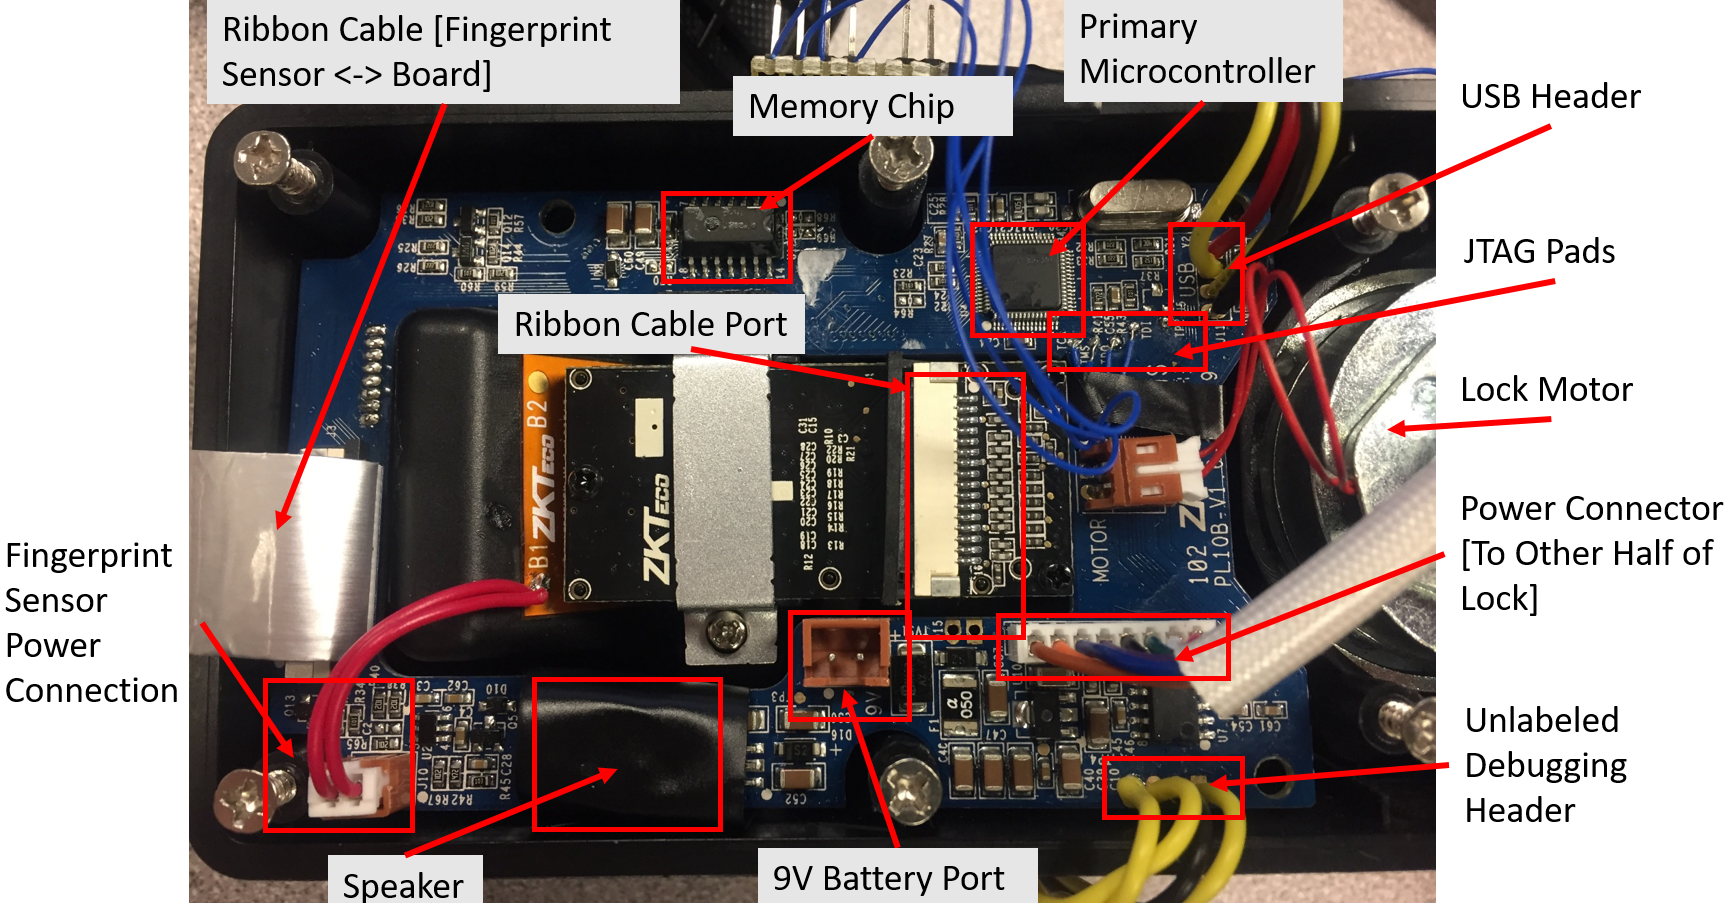
\includegraphics[width=8.7cm]{images/MainPCB(Labeled).png}
  \caption{ZKTeco Primary PCB (Top View)}
  \label{fig:pcb1}
\end{figure}

\bigskip 

In its normal configuration, the door lock can be operated by an authorized user placing a registered fingerprint on the scanner or pressing the unlock button on the mobile app after pairing to and authenticating with the device. Given the appropriate command, the ZKTeco Lock activates a solenoid which causes the external handle to become mechanically bound to the internal latching mechanism, enabling the handle to actuate the latch. When the servo is not activated, the door handle will freely turn without moving the latch. Additionally, if power is lost or the fingerprint scanner and mobile app are not operational, there is a key provided for manual unlock or a port to connect a 9V battery to temporarily charge the lock to grant access to authorized users. Figure \ref{fig:lock} displays the lock breakout and installation guide provided by the manufacturer \cite{ZKTeco}.

\begin{figure}[ht]
  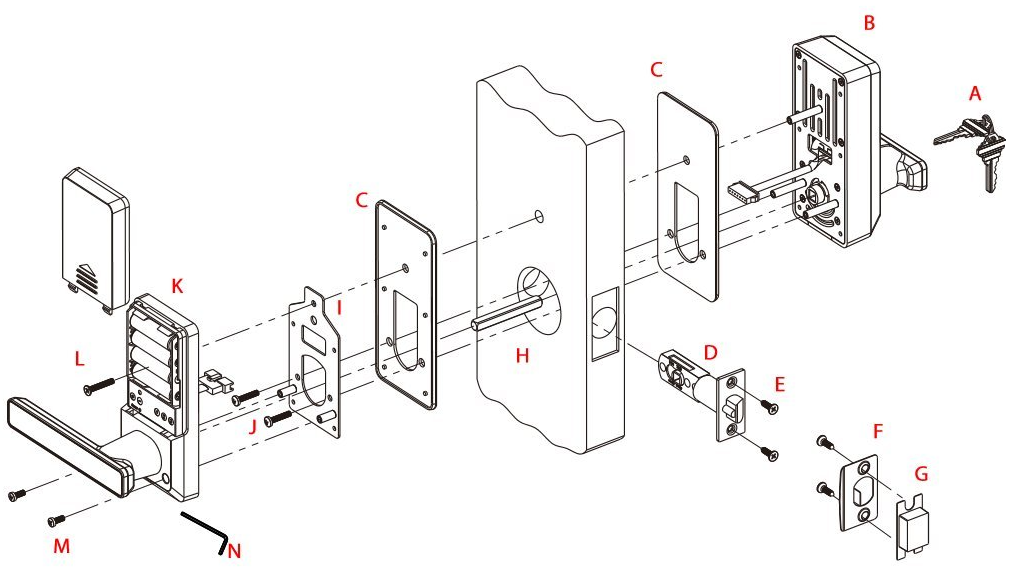
\includegraphics[width=8.5cm]{Lock.png}
  \caption{Smart Lock Breakout}
  \label{fig:lock}
\end{figure}

\bigskip 

A more detailed analysis of the PCB components reveals points of inquiry for deeper analysis and reverse engineering. Several components on the \gls{pcb} are noteworthy: there are two four-pin through hole headers that may be useful for dumping the firmware or performing low-level hardware debugging on the device; one is titled "USB" which could leveraged for easy access to these functions. There are also small pads labeled using the standard convention denoting \gls{jtag} access (TD0, TD1, TMS, TCK, and TP2) as shown in figure \ref{fig:jtag} \cite{IEEE2013}. By removing the \gls{pcb} from the plastic casing access was gained to the Bluetooth \gls{soc}. Finally, We were able to locate a speaker that provides audio feedback to the user, in conjunction with the visual feedback from LEDs.  Because the audio feedback was unnecessary and not conducive to further analysis, electrical tape was applied to prevent distractions.


\begin{figure}[ht]
  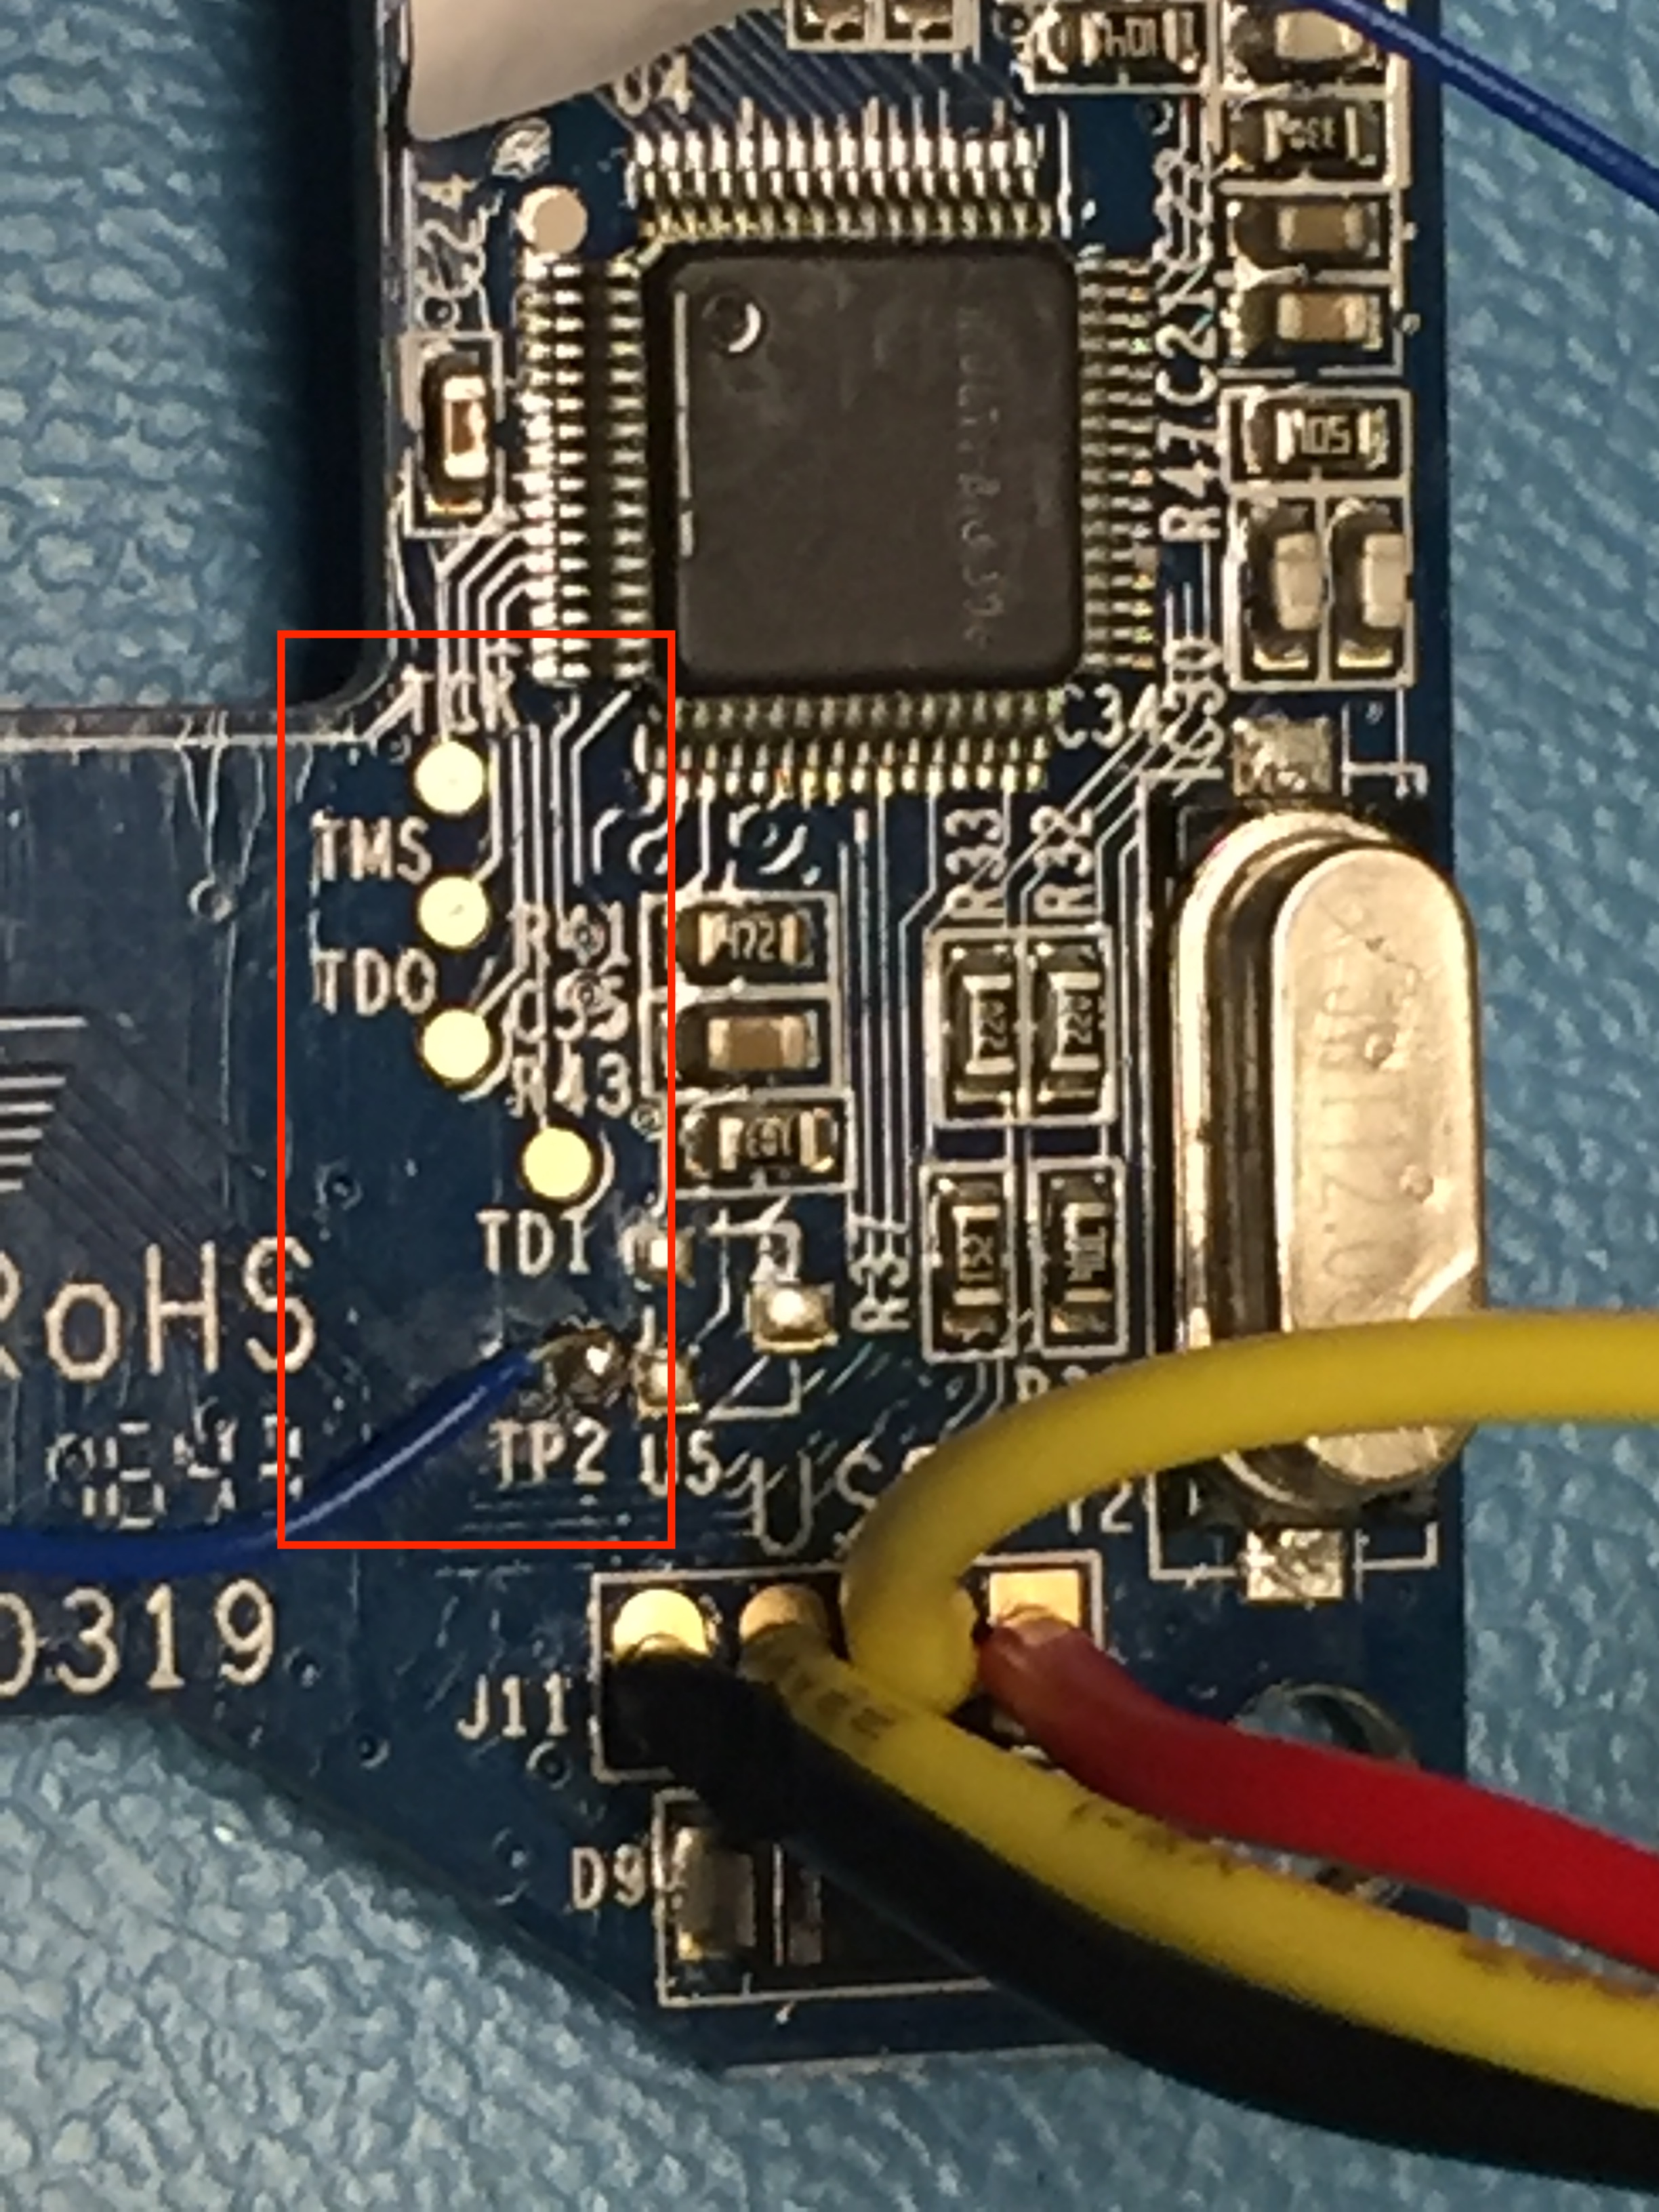
\includegraphics[width=8.5cm]{images/JTAG2.jpg}
  \caption{Labeled JTAG Pads [Magnified]}
  \label{fig:jtag}
\end{figure}

\subsection{Software}

The ZKTeco lock is designed to operate in conjunction with an iOS or Android application that provides authentication and command and control capabilities to the lock mechanism.  As such, it is integral to this effort to understand the behavior of the application.  The testing used two "rooted" Google Pixel smartphones, one "rooted" Google Pixel 2 XL smartphone, and an iPhone 6 running iOS 12.2 as the client controller devices.  Prior to beginning testing operations, each controller had the appropriate version (iOS/Android) of ZK Bio BL v1.1.20 installed.  In a software auditing context, two logical sets of components were identified: the behavior of the mobile app on the controller device, and the communication between the controller and the Bluetooth host device which implements \gls{ble}.

\bigskip
\subsubsection{App Behavior}

Before initiating communications analysis, the general behavior of the Android application was explored.  The audit made use of Android Studio 3.4 on Ubuntu 18.04 to decompress the ZK Bio BL APK and examine its manifest file for permissions information, activities and any associated filters, and notable resources (e.g. pinned certificates).  Additionally, the \gls{adb} was used on the rooted controller devices to examine application-specific files stored on the device.  The final tool used to assist in the exploration of ZK Bio BL app behavior was jadx, which provides Java decompilation capabilities  \cite{Skylot2018} and which can be used to view replicated Java source code to provide insight into the app's internal behavior.  The application was also used according to the manufacturer's instructions to understand its normal modes of operation.

\bigskip
\subsubsection{Bluetooth Communication}

The communication analysis methodology constituted the creation of multiple test cases covering a range of lock and application behaviors and states.  The ZK Bio BL application recognizes 4 distinct user/device roles: \textit{admin}, \textit{user}, \textit{temporary}, and \textit{unauthorized}.  Each role---except unauthorized---is permitted to send an unlock command to the lock.  Additionally, the system permits any type of user to elevate privileges using a superuser-style privilege password.  Test cases were prepared for each user role to initiate initial device pairing with the Bluetooth host, and to elevate privileges into the superuser role.  In addition to using the manufacturer's application to perform communication functions, use was also made of Nordic Semiconductor's nRF Connect app.  This application permits controller devices to audit Bluetooth advertisements, examine services and profiles offered by host devices, and to read and write arbitrary data to characteristic values within advertised attributes that possess readable and writeable properties \cite{NordicSemiconductor}.  Test cases were prepared whereby attempts were made to use nRF connect to mimic ZK Bio BL behavior by sending crafted characteristic value reads and writes.  Finally, failure cases for both the pairing and the permission-elevation procedures were created and analyzed.

\bigskip

In all test cases, the communication was recorded by enabling the BTSnoop logging capabilities provided by the Android operating system \cite{AndroidDevelopers}.  After the required actions were performed on the system, the log was retrieved from the controller device and analyzed with Wireshark - a packet capture and analysis application provided open source \cite{Sharpe}.  Where possible, distinct actions and roles were captured as separate logs.


\section{Analysis}
\subsection{Hardware}

Analysis of the hardware revealed little about the internal working of the lock due to the addition of a conformal coating and the concordant removal of chip identifiers. Both of these significantly hampered several of our analysis threads. Because the main microcontroller and memory chip could not be identified, the firmware remained inaccessible. Figure \ref{fig:ChipText} shows the best view of the identifying markings "MULTI-Bio 306", which do not correspond to any known chip, and which clearly appears to be a manufacturer's, as opposed to foundry's, marking. Even after removal of the conformal coating, no further identifiers were found.  

\begin{figure}[ht]
  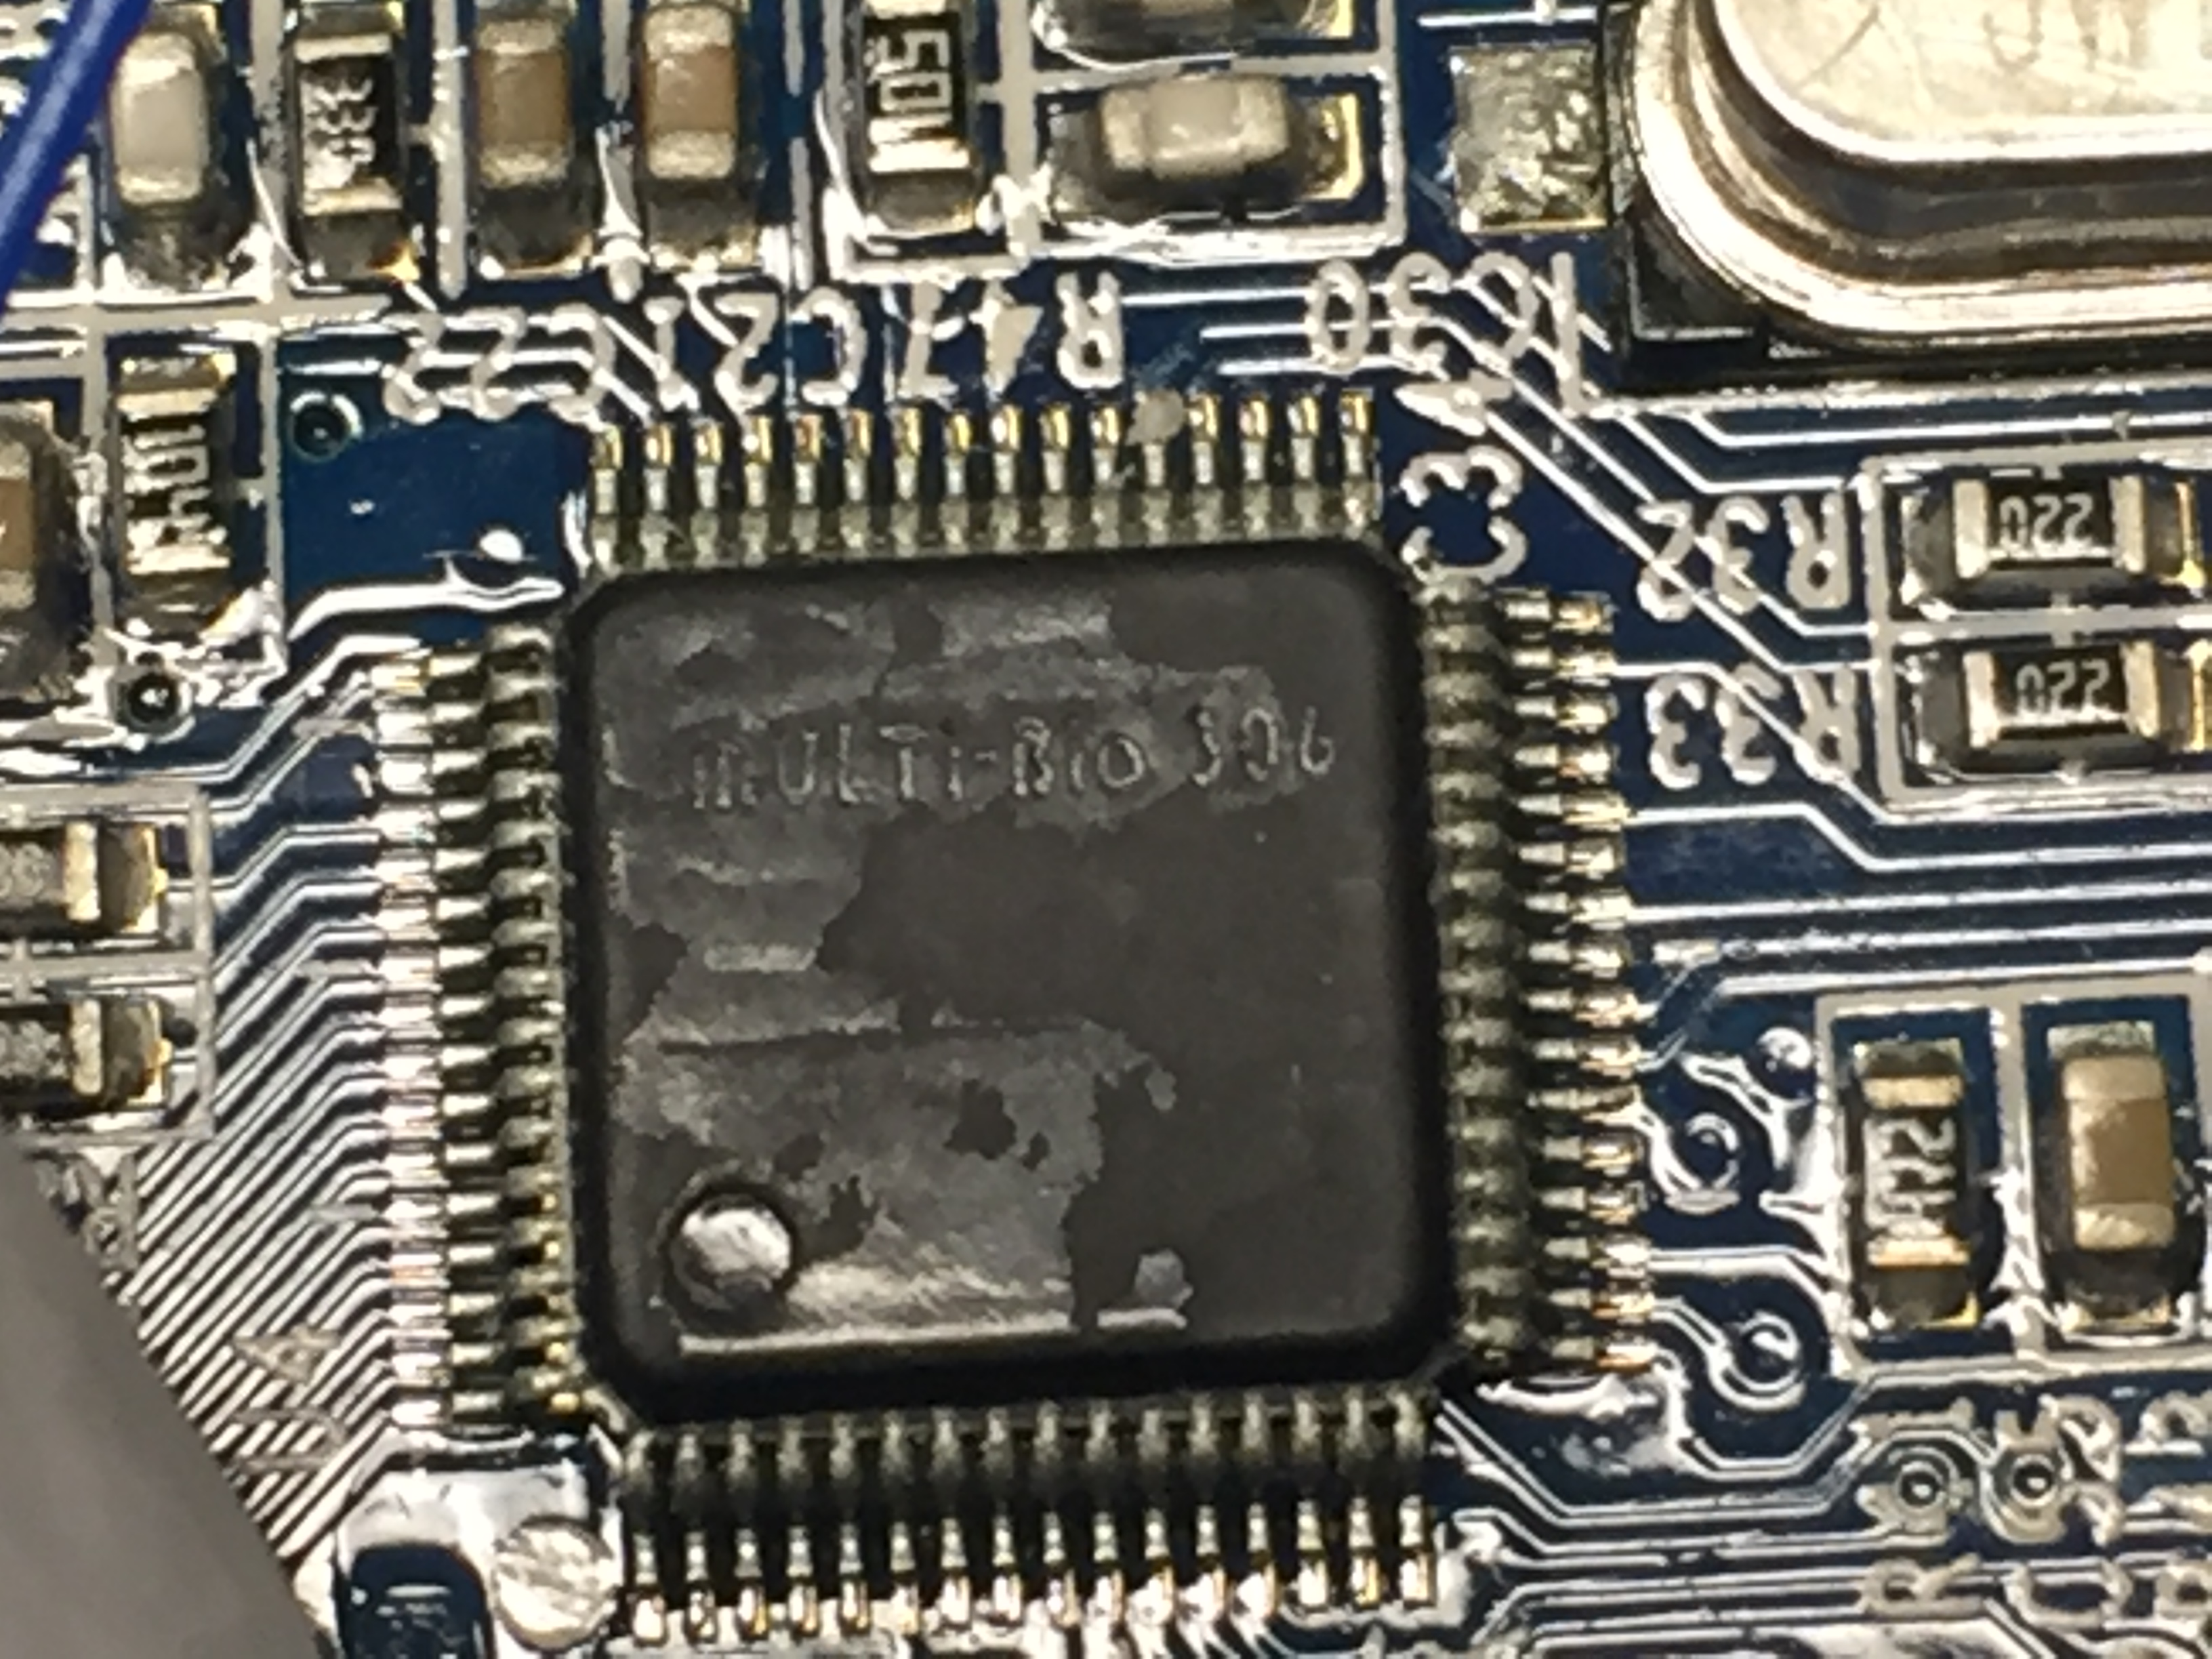
\includegraphics[width=8.5cm]{images/MainChipText.JPG}
  \caption{Primary Microcontroller [Magnified]}
  \label{fig:ChipText}
\end{figure}

The memory chip was also unidentifiable.  Given its size and location on the board it is most likely a non-volatile flash chip storing the firmware.  Figure \ref{fig:memory} shows the most readable view. Both these figures \ref{fig:ChipText} and \ref{fig:memory} show the conformal coating that covers most of the \gls{pcb}. Without verification of the chip architecture and associated pinouts, other hardware analysis was hindered. 

\begin{figure}[ht]
  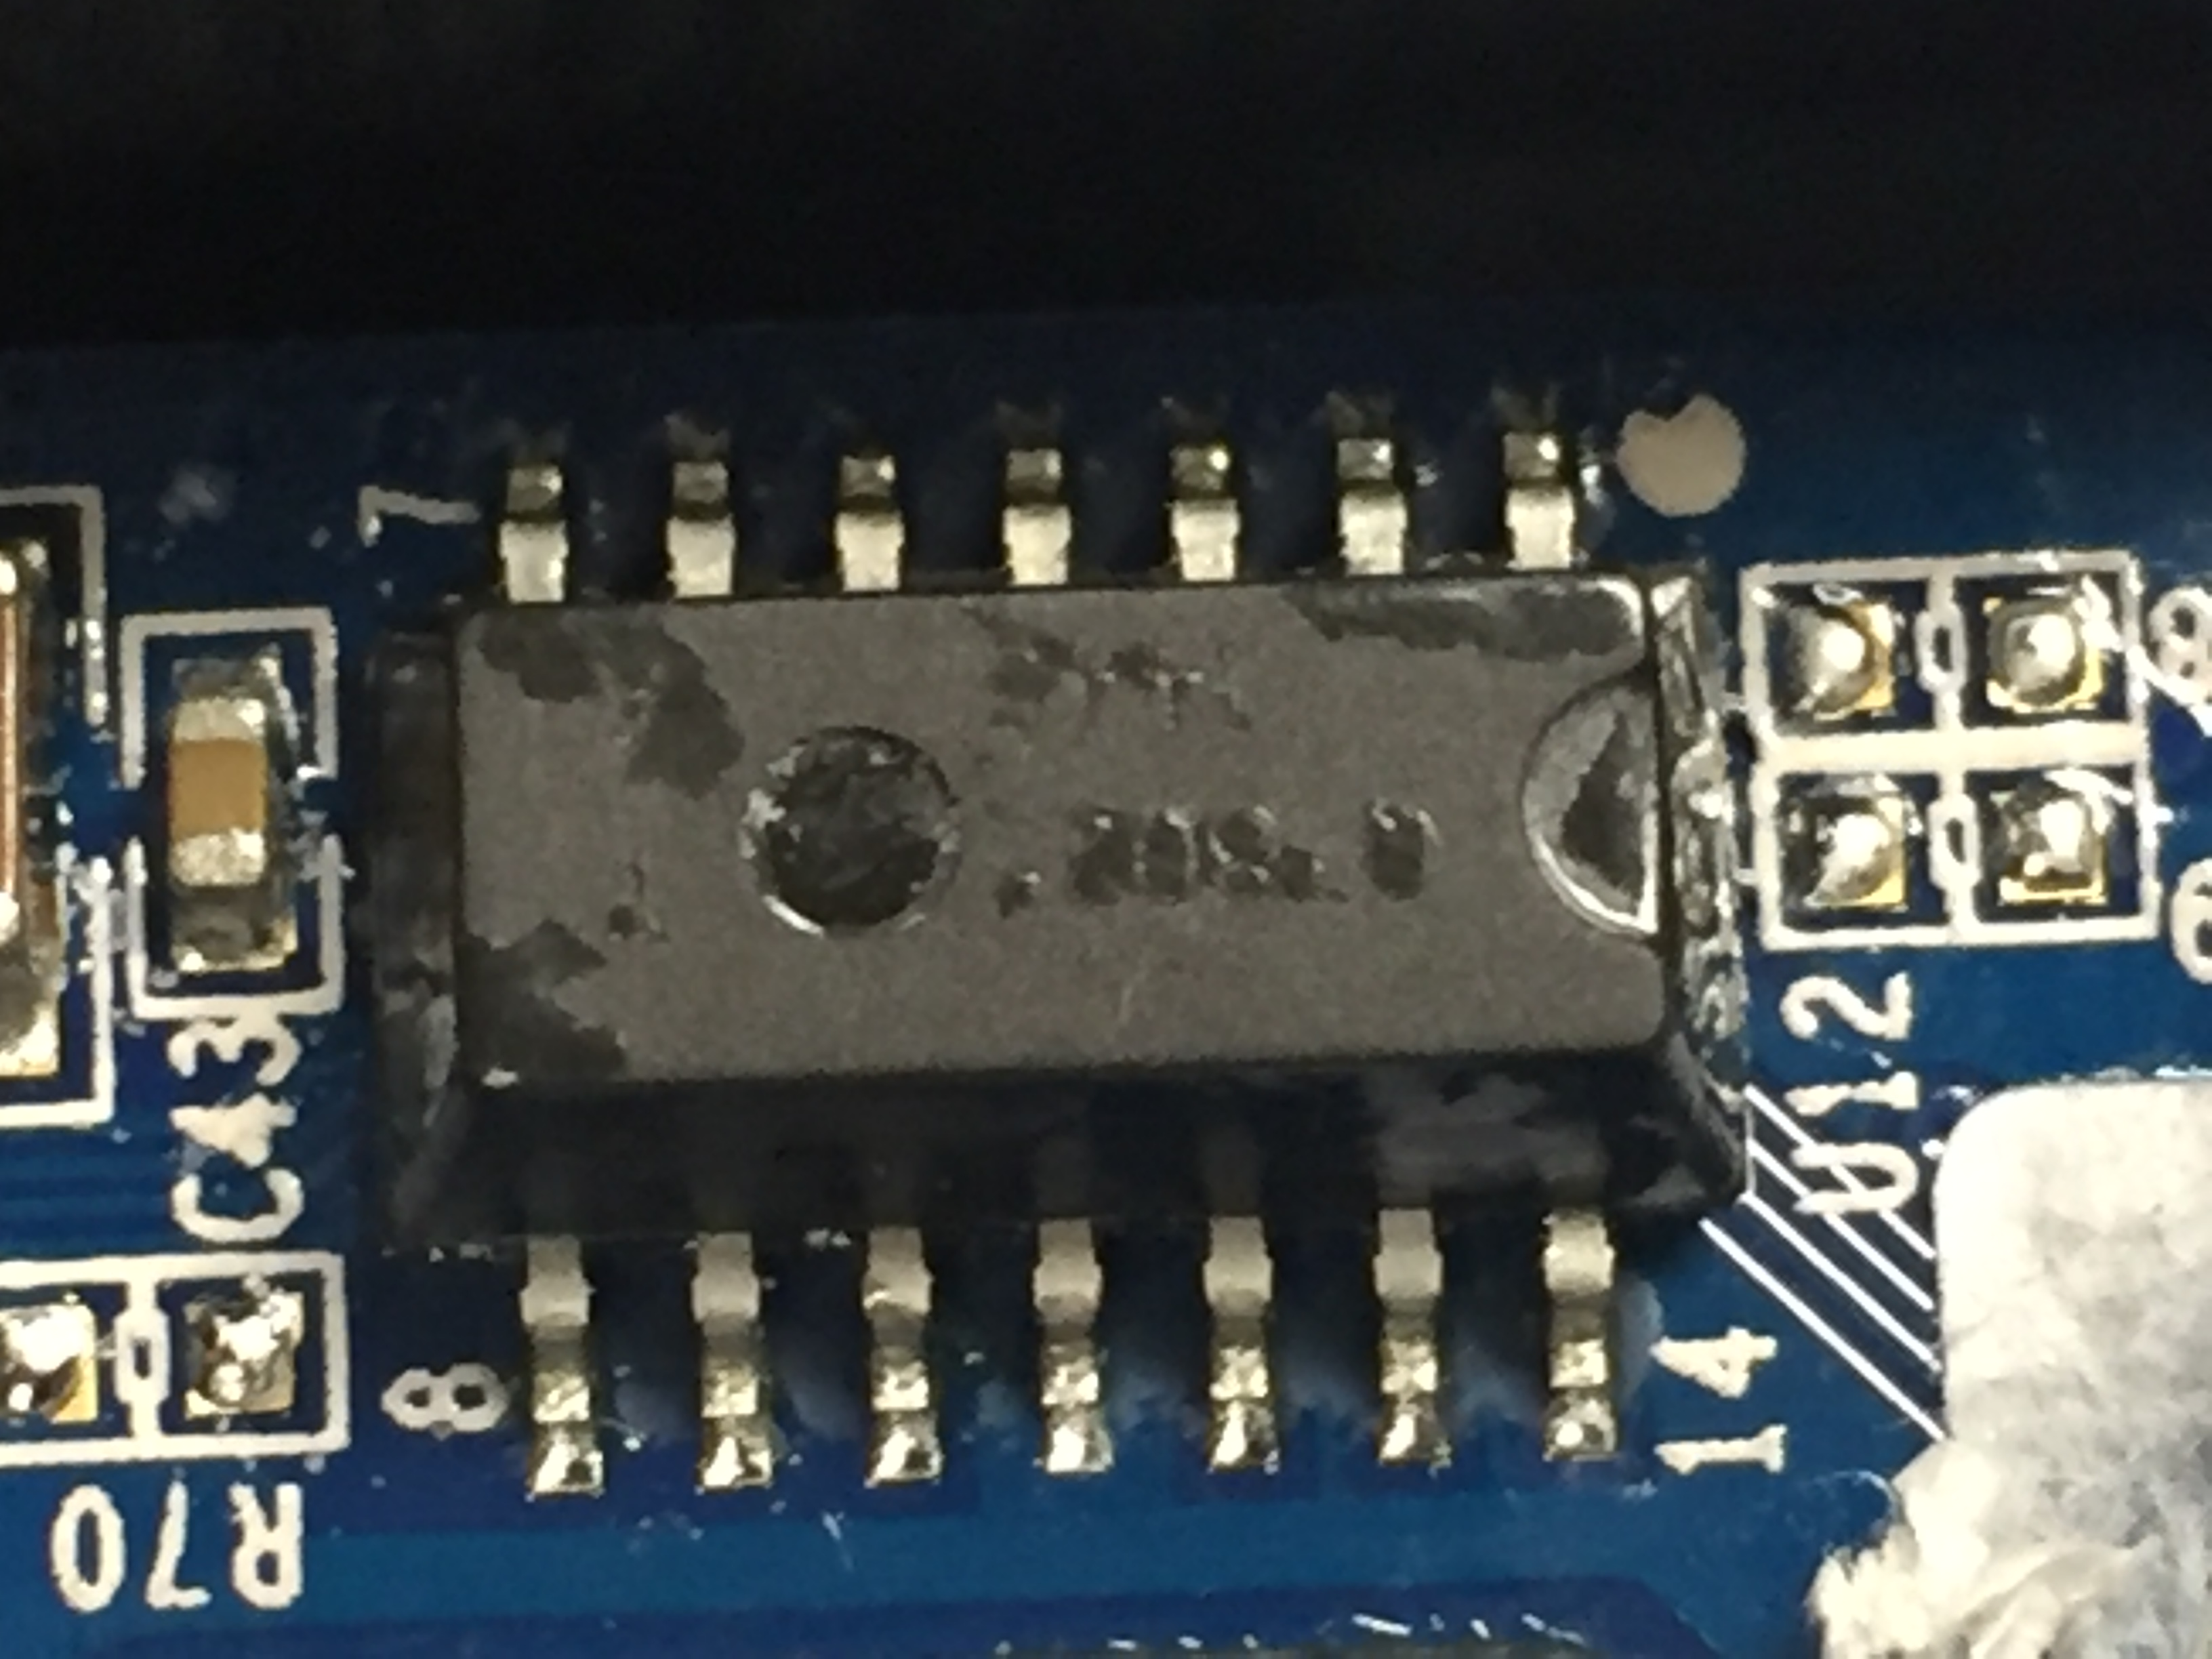
\includegraphics[width=8.5cm]{images/MemoryChip.JPG}
  \caption{Memory Chip [Magnified]}
  \label{fig:memory}
\end{figure}

The \gls{ble} \gls{soc} was well labeled as shown in figure \ref{fig:blechip}. The serial number (DXYBT021) indicated the \gls{ble} \gls{soc} made use of the QN9021 chip package, manufactured by NXP Semiconductors \cite{NXPSemiconductors2018}. 

\begin{figure}[ht]
  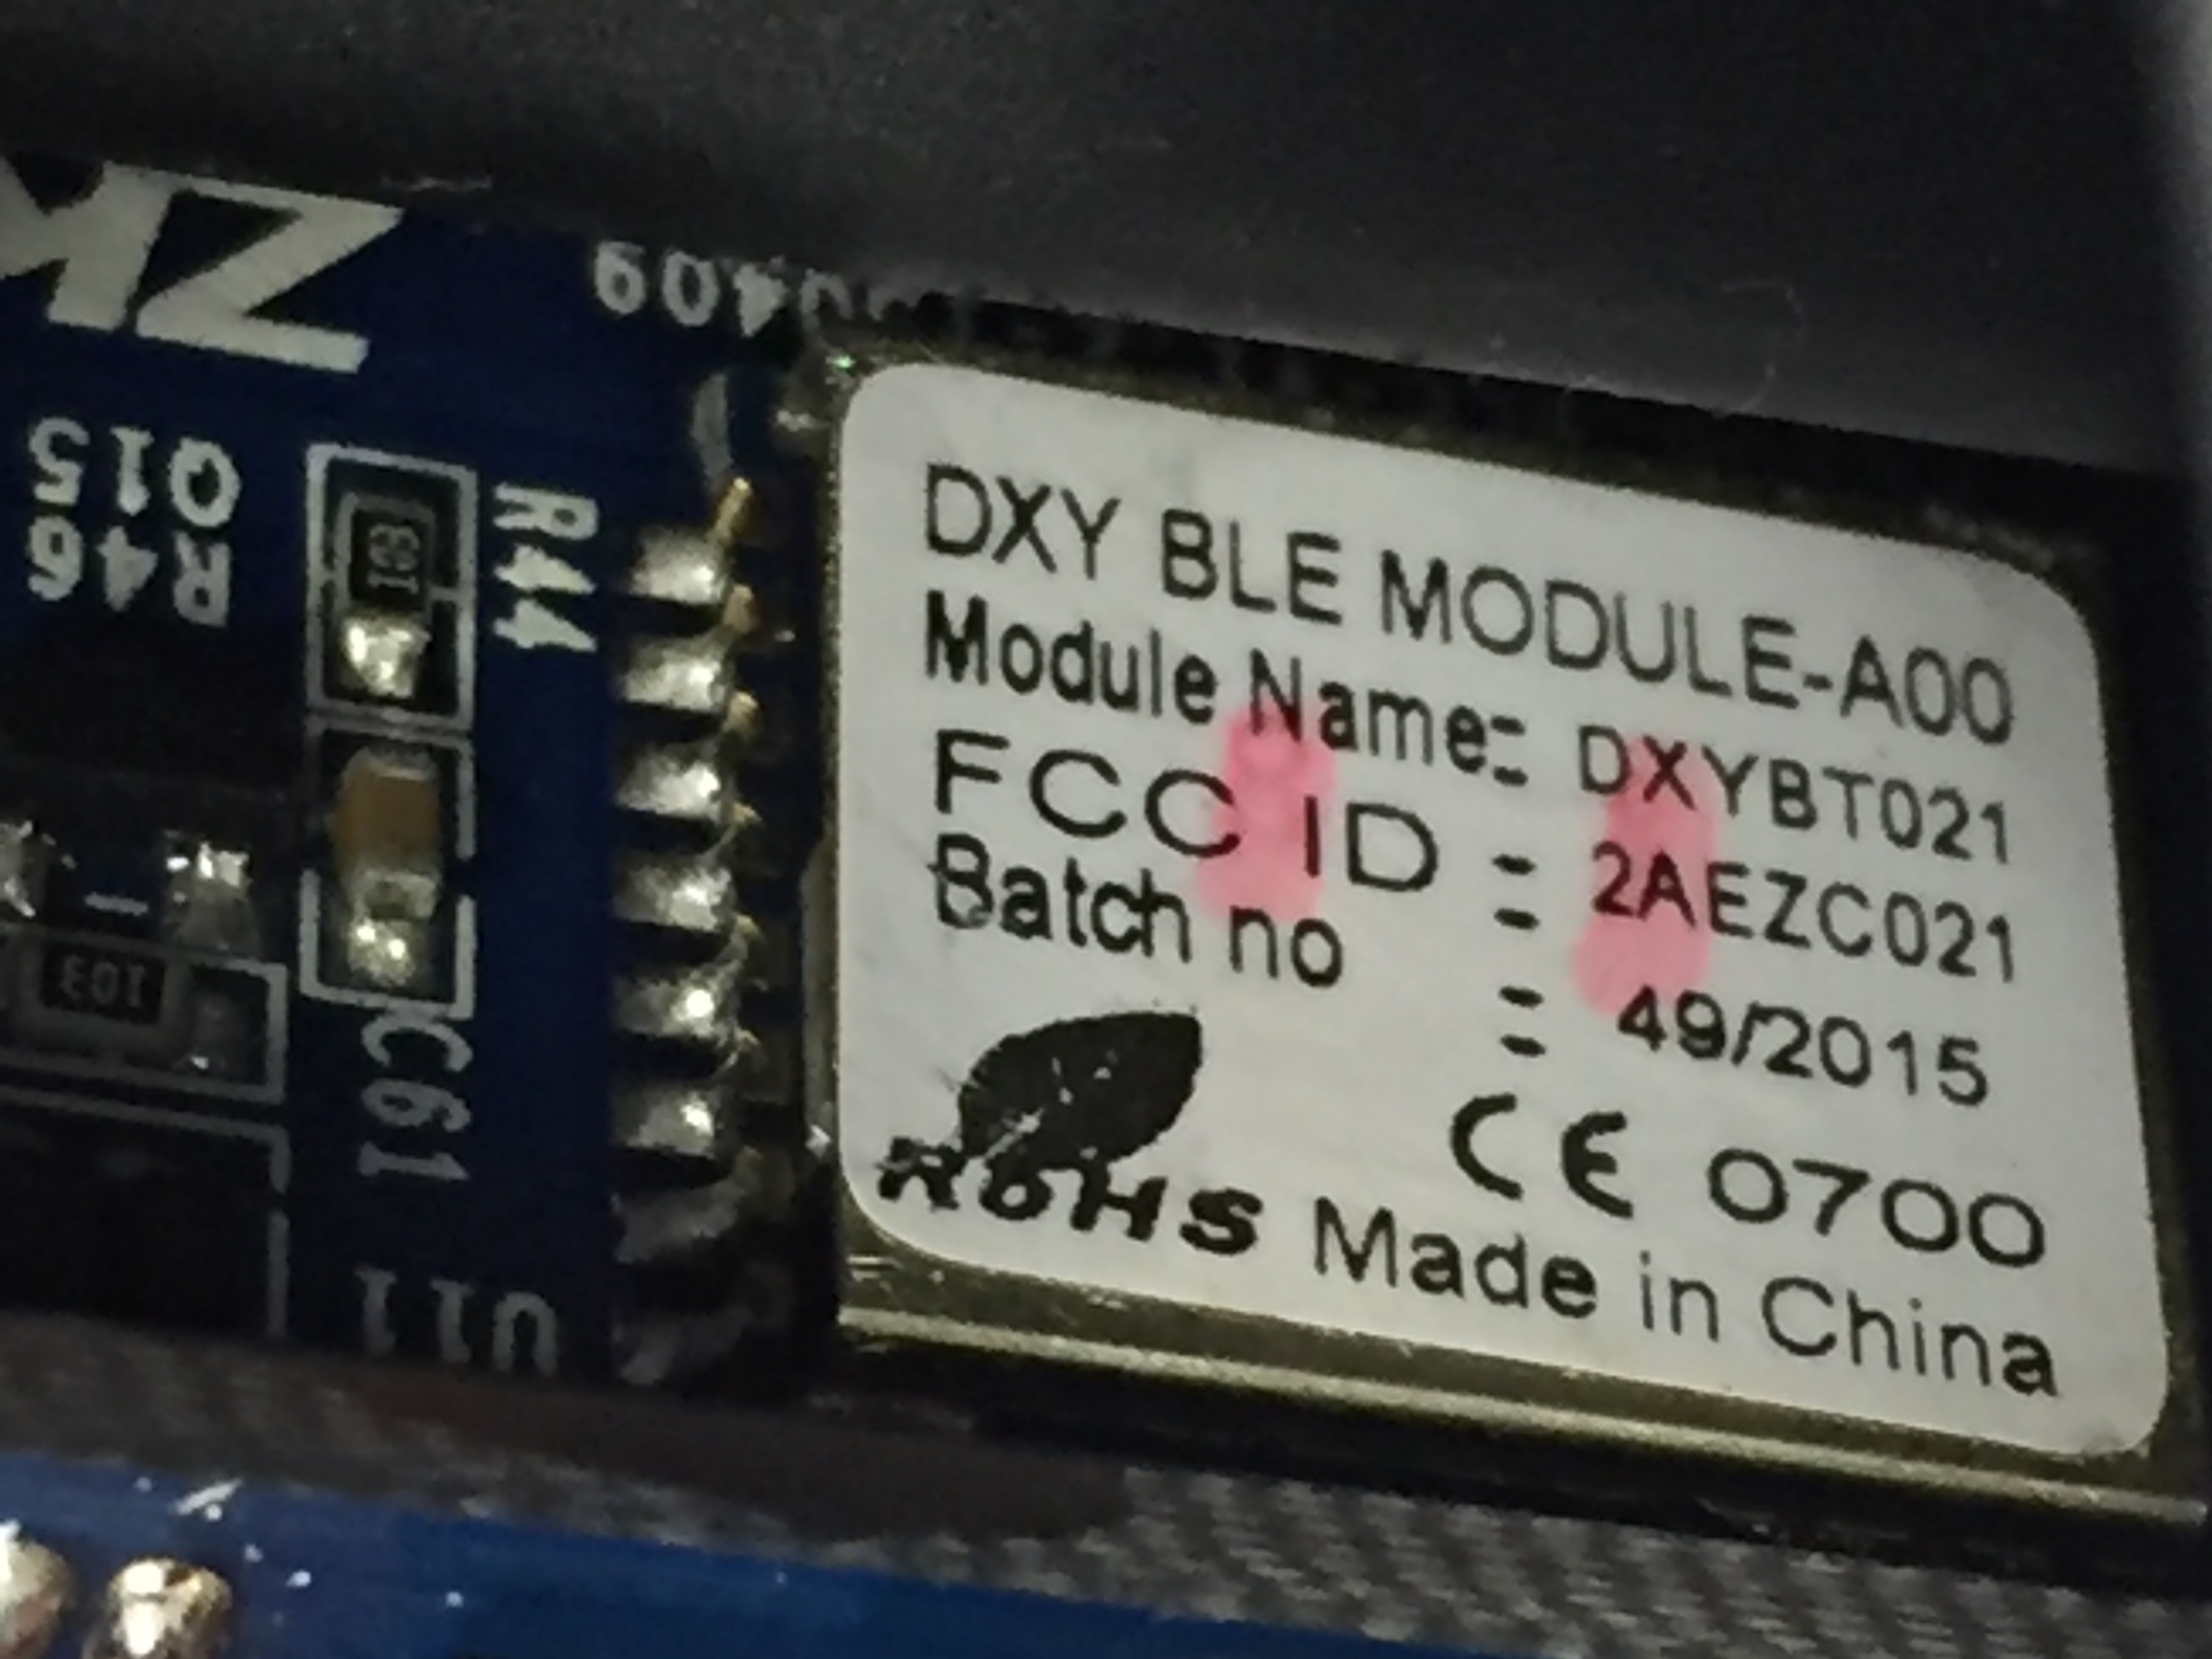
\includegraphics[width=8.5cm]{images/BLEChipText2.jpg}
  \caption{Bluetooth Module Identification Numbers}
  \label{fig:blechip}
\end{figure}

The pinout from the manufacturer website is shown in Figure \ref{fig:blepinout}. Although we had the schematic for this chip, the lack of markings on the board and the connection mechanism between the mainboard and \gls{soc} daughterboard concealed the nature of the connections between the two, and made trace-analysis intractable given the available tools.

\begin{figure}[ht]
  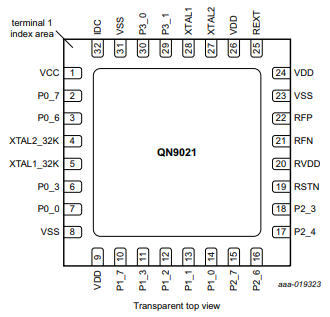
\includegraphics[width=8.5cm]{images/BlueToothChip.png}
  \caption{Bluetooth QN9021 System-On-Chip Pinout}
  \label{fig:blepinout}
\end{figure}

Further analysis revealed that the USB header, \gls{jtag} pads, and the unknown four-pin header were connected to the unidentified, primary microcontroller shown in figure \ref{fig:ChipText}. Although this architecture implied that the microcontroller might expose standard debugging functions and could be accessed accordingly, this was again unsuccessful. Wires were soldered to all three headers and several attempts were made to establish a debugging connection. When the USB header was wired according to the USB standard, the LEDs began the flash, indicating that the header was electrically connected to the rest of the \gls{pcb}. However, no structured data could be detected by a serial connection between the ZKTeco Lock and an Ubuntu 18.04 device. Similarly, no connection could be made to the primary microcontroller via the unknown pins shown in figure \ref{fig:uart}.


\begin{figure}[ht]
  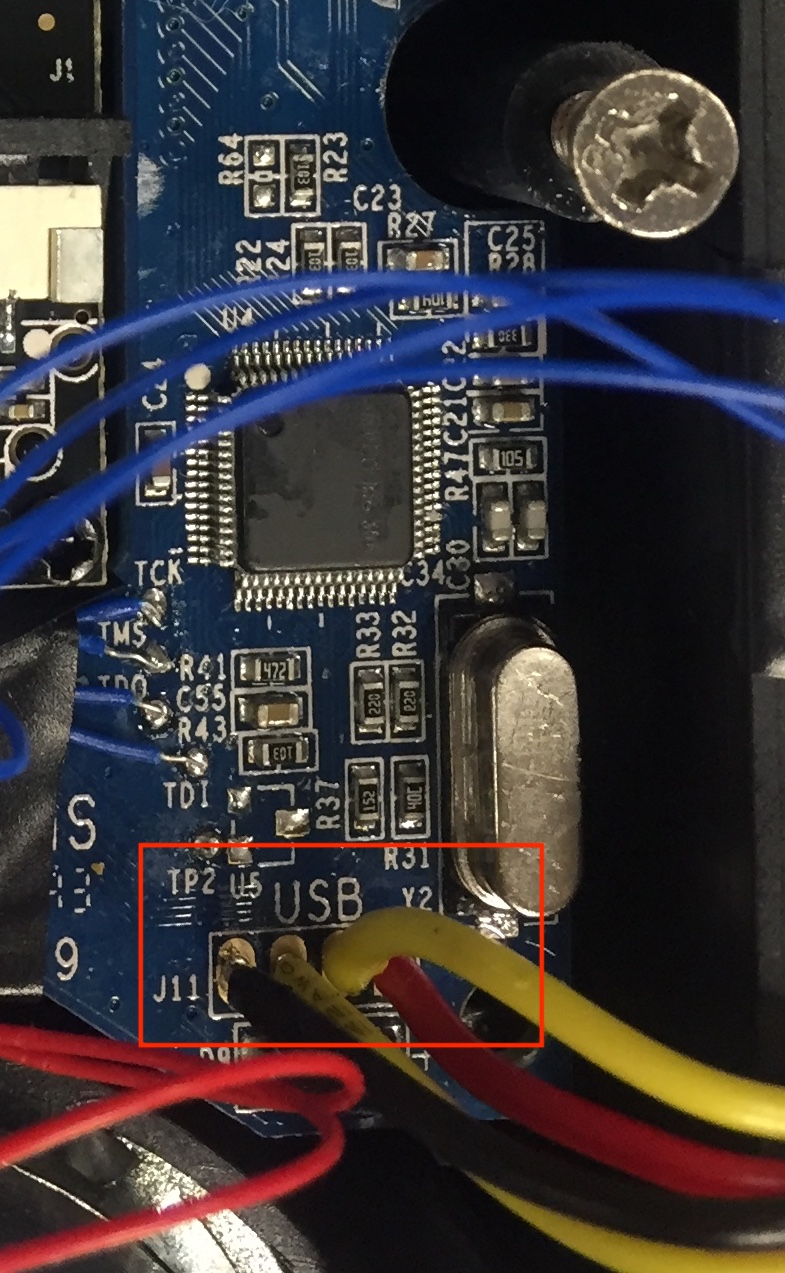
\includegraphics[width=8.5cm]{images/USB.jpeg}
  \caption{USB Interface}
  \label{fig:usb}
\end{figure}

\begin{figure}[ht]
  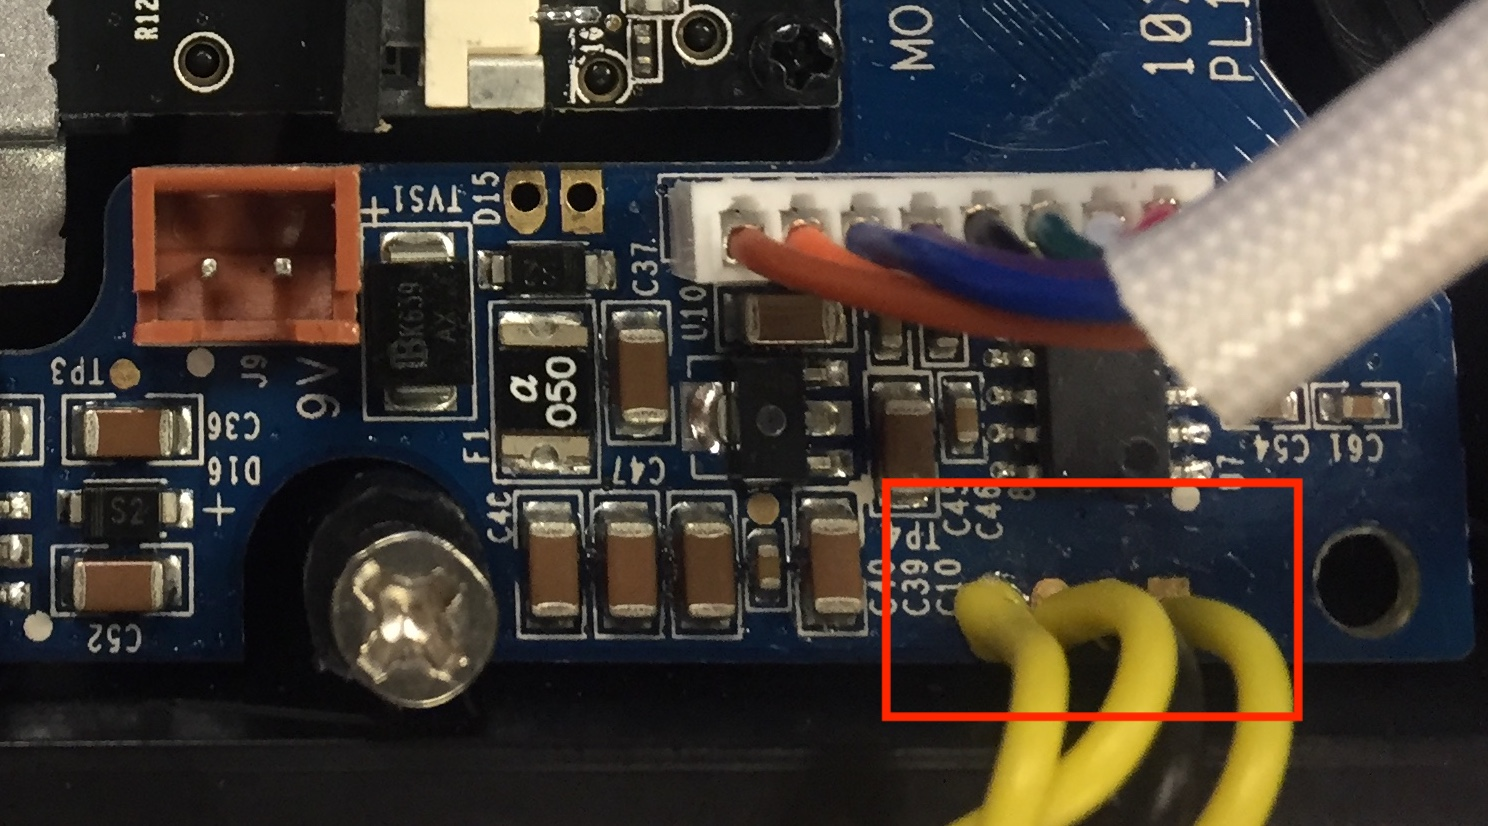
\includegraphics[width=8.5cm]{images/UART.JPG}
  \caption{Unknown Debugging Interface}
  \label{fig:uart}
\end{figure}

\subsection{Software}
\subsubsection{App Behavior}

Application behavior in normal use indicated the developers implemented an idiosyncratic security paradigm for their multi-user lock system.  In particular, the application does not permit any distinction between users and their devices.  User accounts are created only when a new controller device with ZK Bio BL pairs for the first time with a given ZKTeco lock.  On pairing, an \textit{unauthorized} user data object is created in the ZKTeco lock's memory and on the controller device.  This data object has fields for the unique user account ID, user name, user time zone, and a log in ID.  There is no method to associate an existing user account with a new device, nor an existing device with a new user account unless a system user uninstalls the application and re-installs it -- essentially recreating a "new" device.  Because of this behavior, it is neither possible nor useful to distinguish "user" from "device" accounts.

\bigskip

The application provides no means of remotely editing accounts.  That is, account metadata and permissions can only be changed on the specific device associated with that account. As such, all unauthorized users remain in the unauthorized role until the device is physically accessible by a system administrator in possession of the user-configurable superuser passkey.  Once such a system administrator enters the superuser key into the application on the local controller device associated with an account, then that device's account information -- including the user role associated with that account -- can be permanently edited.  On application close, and \textit{only on application close}, the local account loses superuser privileges and reverts to its associated user role (possibly a new role, if one was set during the superuser phase).

\bigskip

Although there are four, distinct semantic labels associated with the account roles, in practice there are only two, functional roles;  Administrators, users, and temporary users can unlock the ZKTeco lock while unauthorized users cannot.  Although marketing information purports that device administrators can perform other, standard administrative functions -- e.g. account creation, per-account privilege scheduling, and security auditing -- these capabilities are either not present or, in the case of account creation, are dependent on entering the superuser key into the appropriate controller device and are wholly unassociated with the account information of the system administrator.

\bigskip

The application makes use of a standard, fairly limited permissions schema that does not appear to have security significance; notable permissions requested include WRITE\_EXTERNAL\_STORAGE, READ\_EXTERNAL\_STORAGE, BLUETOOTH, and BLUETOOTH\_ADMIN.  It also stores relatively little data---which is not surprising given the limited nature of user account management and the application's inability to distinguish users and devices---however, there are still multiple, potential vectors for exploitation.  In particular, the application stores the plaintext pairing key for every lock it has successfully paired with in 

\begin{lstlisting}[caption=information storage location, captionpos=b]
/data/data/com.zktechnology.android.zkbiobl/shared_prefs/DeviceInfo.xml
\end{lstlisting}

Additionally, the \verb|ZKBioBL.xml| in the same location also contains each device's unique key, referred to by the developers as the "InstallMark".  Finally, the application uses a universal, default Bluetooth pairing passkey and administrator password, neither of which are prompted to the user to be changed, either on lock initialization or otherwise.

\bigskip
\subsubsection{Bluetooth Communication}

Since the host device firmware was not obtainable, we could not fully assess the handshaking procedure and develop a holistic model of a complete pairing and unlocking procedure on the ZKTeco lock.  However, multiple features were extracted from which we can derive at least some critical behavior.  Additionally, these features provide reasonable starting points for future investigation.

\bigskip

Like many \gls{ble} \gls{iot} devices, the ZKTeco lock does not implement any native \gls{ble} security pairing mechanism \cite{Newman2019}.  Instead, ZKTeco have elected to permit insecure \gls{ble} connections that then use application logic to authorize command and control from controller devices.  The \gls{ble} handshake uses simple pairing mode most commonly known as "just works mode"  \cite{BluetoothSIG2019}, and connections using 3rd party applications -- like nRF Connect -- are able to successfully complete.  However, connections originating from applications other than ZK Bio BL cause the host device to generate a \verb|remote user terminated connection| Bluetooth disconnect command after 10 seconds unless the device authenticates.

\bigskip

Per the \gls{ble} standard, the host device advertises its capabilities by organizing them in an attribute hierarchy \cite{BluetoothSIG2019}.  The host device advertises one or more \textit{services}; each service consists of one or more field values, known as \textit{characteristics}.  Characteristics possess properties: e.g. \verb|readable, writeable|, and a \textit{value}, denoted by a two-byte handle, that contains that characteristic's data.  All services and characteristics are identified by a 16-byte UUID.  For all Bluetooth Special Interest Group (SIG)-approved services and their component attributes, 14 bytes of the UUID are fixed, and the remaining two bytes function as the unique handle to identify each service.  All vendor-specific services and characteristics require a complete, unique 16-byte UUID which must not use the 14 byte reserved sequence for SIG-approved profiles \cite{BluetoothSIG2019}.

\bigskip

The ZKTeco Lock advertises four services; two of these are SIG-approved, generic services \verb|0x1800 (Generic Access)| and \verb|0x1801 (Generic Attribute)|.  The third is a vendor-specific service associated with Quintic Corp., the \gls{ble} package manufacturer, and does not appear to be of significance.  The final advertised service is a ZKTeco vendor-specific service with UUID \verb|0x00004458-0000-1000-8000-00805f9b34fb|.  It should be noted that this designator uses the reserved 14-byte sequence that normally identifies SIG-approved services, even though the two-byte handle \verb|0x4458| is not associated with any such service.  It appears likely then that the manufacturer re-purposed existing Bluetooth code but changed only a minimal section of the identifier.  A full description of the various services and their characteristics is available in the appendix. The most significant finding is the application's use of characteristics \verb|0x4459| and \verb|0x4460| of the \verb|0x4458| service.  Characteristic \verb|0x4459| holds a 20-byte value at handle \verb|0x0019| that is read in by the host device for authenticating the privilege password; while characteristic \verb|0x4460| holds a 19-byte value at handle \verb|0x001c| that is read in by the host device for authenticating the pairing passkey.  Writing to these handles with the appropriate authentication information is critical to maintaining a connection and preventing the host device from terminating the communication. 

\bigskip
\subsubsection{Authentication}

The application uses three authentication or pseudo-authentication mechanisms prior to issuing an unlock command to the appropriate attribute: (pairing) passkey, a privilege password, and the unique "InstallMark" device identifier.  After performing a \gls{ble} simple pairing between the ZKTeco lock host and a controller device, the controller first writes to the Client Characteristic Configuration attributes associated with these two characteristics (using handled \verb|0x001a| and \verb|0x001d|, respectively) to enable notification from the host after the associated values are written; this configuration change is required for the ZK Bio BL application to properly "pair".   After the configuration change, the handshake proceeds as in fig. \ref{fig:handshake}.

\begin{figure}[ht]
  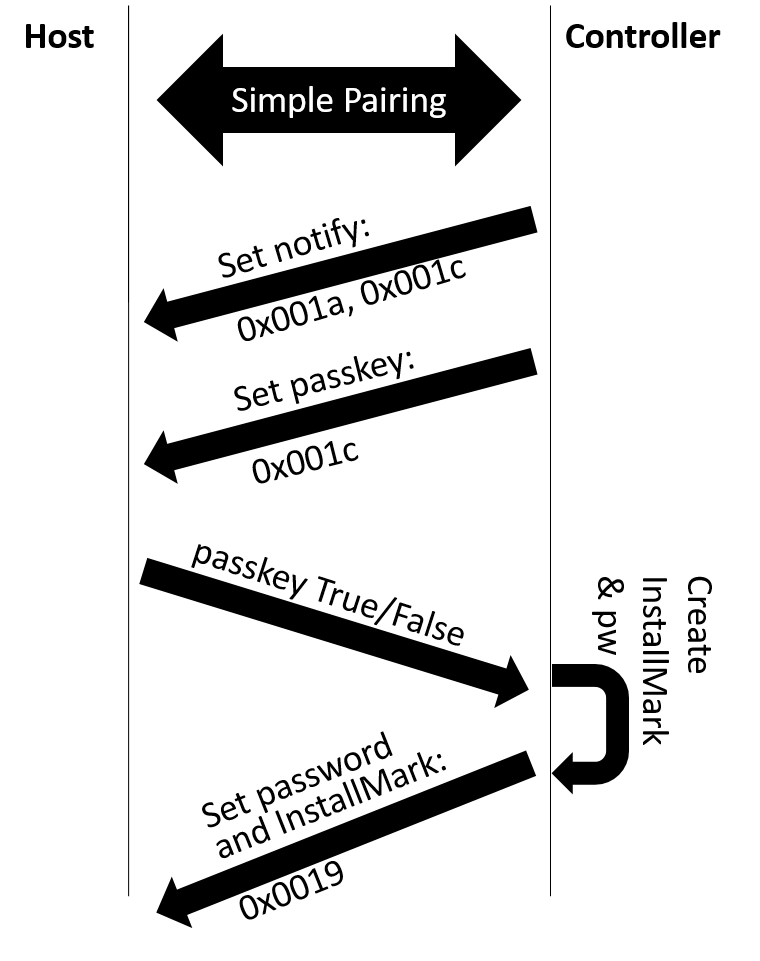
\includegraphics[width=\columnwidth]{/handshake.png}
  \caption{\gls{ble} handshake}
  \label{fig:handshake}
\end{figure}

\bigskip 

After the controller application processes the initial simple pairing connection request, the local application begins a three-step process.  It first sends a \gls{ble} write command to handle \verb|0x001c| with the pairing passkey.  If the lock has not yet been configured with a key, a default value of "1234" is passed, in either case the application formats the passkey \verb|nnnnnn| into the plaintext string \verb|AT+PASSKEY=nnnnnn|.  The application then checks the controller handle value notification to see if it contains the plaintext response \verb|PASSKEY TRUE|.  If this check fails, the connection is severed \textit{by the controller application}.  If this check passes, then the controller saves the pin in the \verb|DeviceInfo.xml| shared\_prefs file.

\bigskip

Once the appropriate response to the passkey is received and processed, then the next step of the handshake proceeds and the host application looks for a privilege password to set the user privilege level -- this is either the superuser password or, if not entered, a static value hard-coded into the application: \verb|12312124234|.  If the user has not provided the superuser password, the application provides the user password without additional intervention.  This password technically constitutes the second authentication check, though necessarily a fairly poor one.

\bigskip

This password is passed by the application into a method that constructs a larger object containing it, an address corresponding to the connection handle formatted into a 6-byte address (e.g. handle \verb|0x02| formats as \verb|0x02:00:00:00:00:00|) and a unique device identifier.  Since all values are passed in plaintext, they are observable to any eavesdropper within the operating range of the Bluetooth system.  The unique identifier---"InstallMark"---is first checked for in the\verb|ZKBioBL.xml| file.  If not present, it is constructed by the application using the following Java algorithm:

\lstinputlisting[language=java, caption=InstallMark Creation Algorithm, captionpos=b]{InstallMarkCode.txt}

It is unclear if this algorithm, in particular the manner in which the digest is used, represents a meaningful procedure.

\bigskip

Finally, the controller passes the concatenated value \verb|password\nBThandle-InstallMark| to handle \verb|0x0019|.  If the password and InstallMark values pass an unknown check on the host device, then the controller application is permitted to request data from the ZKTeco lock and to send an unlock command to it.  This handshake must take less than 10 seconds or the host device will terminate the connection.

\section{Conclusion}

The analysis described above reveals multiple potential vulnerabilities in the ZKTeco Lock. However, the manufacturer's decision to employ a conformal coating that obscured architectural details was, intentionally or otherwise, effective at preventing attempts to reverse engineer the system.  Correspondingly, the effect is preserved by the manufacturer's decision not to provide firmware or a firmware update procedure.  This is, however, almost certainly a poor long-term security strategy \cite{Rescorla2003}.  In the event a firmware vulnerability is discovered, all PL-10B locks would be rendered permanently insecure.  Although the ZK Bio BL software did use ProGuard to obfuscate the code \cite{AndroidDevelopers}, as with the hardware obfuscation this only hinders---not prevents---vulnerability exploitation.  In particular, the software shows potential vulnerability in both the security model and assumptions, and in decisions made in security implementation in code.

\subsection{Potential Vulnerabilities}
\subsubsection{Security Assumptions}

Examination of the software and methods of lock administration revealed a physical access vulnerability. The use of default passwords poses a known security risk \cite{Fraunholz2017}\cite{Niemietz2015}, but the manufacturer programs every lock with default superuser password and Bluetooth passkey.  These defaults are easily accessible to a malicious actor, and this vulnerability is magnified by the fact that the user is not prompted to change either code during initialization and must navigate through the app to find the correct option.  Furthermore, an attacker who exploited this vulnerability could erase all the current authorized users -- denying service to current users while unlocking the lock at a time of their choosing. Similarly, If a user only uses a mobile device to operate and manage the lock, without adding their fingerprint to the access list their device will also be vulnerable. This would create a situation where the first person to use the fingerprint scanner could be added to the administrator access list. This attack vector seems less likely than the first, but is still possible.

\bigskip

These vulnerabilities emphasize that device security consists of more than the implementation of hardware, software, and data security mechanisms, but must also engage with user training and software enforcement of best practices -- especially in an \gls{iot} context. Vulnerabilities were introduced alongside parallel administrative and security mechanisms. The decision to have distinct access mechanisms created a situation where the user must secure each avenue of access to ensure the highest level of security.

\bigskip

There are several actions the manufacturer could take to protect their users against these vulnerabilities. First, each device should be sent from the factory with a unique default pairing and administrator codes. This would require a malicious actor to obtain the specific codes provided with the device. This would also protect users who never used a mobile app to connect to the lock. Additionally, the app could be programmed to force the user to change the default codes during the first use  \cite{Fraunholz2017}\cite{Niemietz2015}.

\bigskip
\subsubsection{Code Vulnerabilities}

The largest potential vulnerability in the ZKTeco Lock is the developer's decision to use \gls{ble} simple pairing mode and neglecting to enable an encrypted, authenticated pairing \cite{Quinn2019}.  This failure allows a malicious actor to eavesdrop on all \gls{ble} communication and retrieve the Bluetooth passkey, superuser or user password, and device unique identifiers from any simple communication between a legitimate user and the ZKTeco Lock.  Additionally, the ZKTeco Lock always returns account information related to the controller device during the initial communication -- prior to any unlocking request -- so an attacker can obtain account names, IDs, and PINs without any active scanning or exploitation.

\bigskip

Finally, the manufacturer's attempt to develop their own security algorithms to authenticate a device handshake is insecure.  Vulnerabilities are commonly introduced by attempts to develop custom 'cryptographic' protocols \cite{Chatzikonstantinou2016}, and although the developer does use the Java MD5 implementation, they store the derived device key insecurely, transmit it insecurely, and use no random seed.  In theory, this vulnerability should be minor, as replicating an existing unique ID requires accessing information protected by the Android operating system.  However, the plaintext handshake means unique IDs can be passively sniffed with little difficulty.  Had the developer used \gls{ble} encrypted pairing, device IDs could have been securely generated \cite{Chatzikonstantinou2016} and securely transmitted.

\subsection{Future Work}

There are ample opportunities for developing and expanding on the findings of this paper.  Low level reverse engineering efforts using oscilloscopes or logic analyzers to gain access to a firmware dump through the \gls{jtag} pads or USB headers have been successfully used against similar targets in the past \cite{REinIoT}\cite{Barcena2015} and could permit a more complete understanding of the authentication protocol used by ZKTeco.  Additionally, although code obfuscation made traces difficult to parse, code injection using tools like Frida could provide the ability to read parameters and returns from relevant functions to validate authentication behavior \cite{NowSecure}.  Since handshaking authentication is enforced by the application properly responding to a \verb|PASSKEY FALSE| characteristic value read, Frida injection could potentially allow the lock to be exploited with any Bluetooth passkey.  Finally, a similar exploit could be implemented by programming an Android application to mimic the handshake but fail to perform the requisite checks, or by using a Man-in-the-Middle Bluetooth proxy to intercept and mutate packets.


% use section* for acknowledgment
% \section*{Acknowledgment}


% The authors would like to thank...

% references section
\printbibliography[title={References}]


\clearpage
\begin{landscape}
\appendix[GATT SERVICES]

\begin{table}[ht]
\renewcommand{\arraystretch}{1.3}
\begin{tabular}{@{}llllllll@{}}
\toprule
Service Handle              & Service UUID                & Characteristic Handle        & Char UUID                    & Attribute (ATT) Name                                                                   & ATT Handle               & ATT UUID                         & \begin{tabular}[c]{@{}l@{}}Properties\\   (Read, Write, Write without Response,\\   Notify, Indicate)\end{tabular} \\ \midrule
\rowcolor[HTML]{3166FF} 
{\color[HTML]{000000} 0001} & {\color[HTML]{000000} 1800} & {\color[HTML]{000000} }      & {\color[HTML]{000000} }      & {\color[HTML]{000000} }                                                                & {\color[HTML]{000000} }  & {\color[HTML]{000000} }          & {\color[HTML]{000000} }                                                                                            \\
                            &                             & \cellcolor[HTML]{FFFE65}0002 & \cellcolor[HTML]{FFFE65}2803 & \cellcolor[HTML]{FFFE65}                                                               & \cellcolor[HTML]{FFFE65} & \cellcolor[HTML]{FFFE65}         & \cellcolor[HTML]{FFFE65}                                                                                           \\
                            &                             &                              &                              & Device Name                                                                            & 0003                     & 2a00                             & R, W                                                                                                               \\
                            &                             & \cellcolor[HTML]{FFFE65}0004 & \cellcolor[HTML]{FFFE65}2803 & \cellcolor[HTML]{FFFE65}                                                               & \cellcolor[HTML]{FFFE65} & \cellcolor[HTML]{FFFE65}         & \cellcolor[HTML]{FFFE65}                                                                                           \\
                            &                             &                              &                              & Appearance                                                                             & 0005                     & 2a01                             & R                                                                                                                  \\
                            &                             & \cellcolor[HTML]{FFFE65}0006 & \cellcolor[HTML]{FFFE65}2803 & \cellcolor[HTML]{FFFE65}                                                               & \cellcolor[HTML]{FFFE65} & \cellcolor[HTML]{FFFE65}         & \cellcolor[HTML]{FFFE65}                                                                                           \\
                            &                             &                              &                              & Peripheral Privacy Flag                                                                & 0007                     & 2a02                             & R, W                                                                                                               \\
                            &                             & \cellcolor[HTML]{FFFE65}0008 & \cellcolor[HTML]{FFFE65}2803 & \cellcolor[HTML]{FFFE65}                                                               & \cellcolor[HTML]{FFFE65} & \cellcolor[HTML]{FFFE65}         & \cellcolor[HTML]{FFFE65}                                                                                           \\
                            &                             &                              &                              & \begin{tabular}[c]{@{}l@{}}Peripheral Preferred Connection\\   Parameters\end{tabular} & 0009                     & 2a04                             & R                                                                                                                  \\
                            &                             & \cellcolor[HTML]{FFFE65}000a & \cellcolor[HTML]{FFFE65}2803 & \cellcolor[HTML]{FFFE65}                                                               & \cellcolor[HTML]{FFFE65} & \cellcolor[HTML]{FFFE65}         & \cellcolor[HTML]{FFFE65}                                                                                           \\
                            &                             &                              &                              & Reconnection Address                                                                   & 000b                     & 2a03                             & R, W, W(xr)                                                                                                        \\
\rowcolor[HTML]{3166FF} 
{\color[HTML]{000000} 000c} & {\color[HTML]{000000} 1801} & {\color[HTML]{000000} }      & {\color[HTML]{000000} }      & {\color[HTML]{000000} }                                                                & {\color[HTML]{000000} }  & {\color[HTML]{000000} }          & {\color[HTML]{000000} }                                                                                            \\
                            &                             & \cellcolor[HTML]{FFFE65}000d & \cellcolor[HTML]{FFFE65}2803 & \cellcolor[HTML]{FFFE65}                                                               & \cellcolor[HTML]{FFFE65} & \cellcolor[HTML]{FFFE65}         & \cellcolor[HTML]{FFFE65}                                                                                           \\
                            &                             &                              &                              & Service Changed                                                                        & 000e                     & 2a05                             & R, I                                                                                                               \\
                            &                             &                              &                              & Client Characteristic Configuration                                                    & 000f                     & 2902                             &                                                                                                                    \\
\rowcolor[HTML]{3166FF} 
{\color[HTML]{000000} 0010} & {\color[HTML]{000000} fee8} & {\color[HTML]{000000} }      & {\color[HTML]{000000} }      & {\color[HTML]{000000} }                                                                & {\color[HTML]{000000} }  & {\color[HTML]{000000} }          & {\color[HTML]{000000} }                                                                                            \\
                            &                             & \cellcolor[HTML]{FFFE65}0011 & \cellcolor[HTML]{FFFE65}2803 & \cellcolor[HTML]{FFFE65}                                                               & \cellcolor[HTML]{FFFE65} & \cellcolor[HTML]{FFFE65}         & \cellcolor[HTML]{FFFE65}                                                                                           \\
                            &                             &                              &                              & Value                                                                                  & 12                       & 003784cff7e355b46c4c9fd140100a16 & N                                                                                                                  \\
                            &                             &                              &                              & Client Characteristic Configuration                                                    & 13                       & 2902                             &                                                                                                                    \\
                            &                             &                              &                              & Char description                                                                       & 14                       & 2901                             &                                                                                                                    \\
                            &                             & \cellcolor[HTML]{FFFE65}0015 & \cellcolor[HTML]{FFFE65}2803 & \cellcolor[HTML]{FFFE65}                                                               & \cellcolor[HTML]{FFFE65} & \cellcolor[HTML]{FFFE65}         & \cellcolor[HTML]{FFFE65}                                                                                           \\
                            &                             &                              &                              & Value                                                                                  & 16                       & 013784cff7e355b46c4c9fd140100a16 & W(xr)                                                                                                              \\
\rowcolor[HTML]{3166FF} 
{\color[HTML]{000000} 0017} & {\color[HTML]{000000} 4458} & {\color[HTML]{000000} }      & {\color[HTML]{000000} }      & {\color[HTML]{000000} }                                                                & {\color[HTML]{000000} }  & {\color[HTML]{000000} }          & {\color[HTML]{000000} }                                                                                            \\
                            &                             & \cellcolor[HTML]{FFFE65}0018 & \cellcolor[HTML]{FFFE65}2803 & \cellcolor[HTML]{FFFE65}                                                               & \cellcolor[HTML]{FFFE65} & \cellcolor[HTML]{FFFE65}         & \cellcolor[HTML]{FFFE65}                                                                                           \\
                            &                             &                              &                              & Unknown                                                                                & 0019                     & 4459                             & W, W(xr), N                                                                                                        \\
                            &                             &                              &                              & Client Characteristic Configuration                                                    & 001a                     & 2902                             &                                                                                                                    \\
                            &                             & \cellcolor[HTML]{FFFE65}001b & \cellcolor[HTML]{FFFE65}2803 & \cellcolor[HTML]{FFFE65}                                                               & \cellcolor[HTML]{FFFE65} & \cellcolor[HTML]{FFFE65}         & \cellcolor[HTML]{FFFE65}                                                                                           \\
                            &                             &                              &                              & Unknown                                                                                & 0001c                    & 4460                             & W, W(xr), N                                                                                                        \\
                            &                             &                              &                              & Client Characteristic Configuration                                                    & 001d                     & 2902                             &                                                                                                                    \\ \bottomrule
\end{tabular}
\caption{ZKTeco Lock \gls{ble} ATT Profile.  Services are in red, their characteristics in yellow, and attributes uncolored}
\label{tab:att}
\end{table}
\end{landscape}


% *** GRAPHICS RELATED PACKAGES ***
%
\ifCLASSINFOpdf
  % \usepackage[pdftex]{graphicx}
  % declare the path(s) where your graphic files are
  % \graphicspath{{../pdf/}{../jpeg/}}
  % and their extensions so you won't have to specify these with
  % every instance of \includegraphics
  % \DeclareGraphicsExtensions{.pdf,.jpeg,.png}
\else
  % or other class option (dvipsone, dvipdf, if not using dvips). graphicx
  % will default to the driver specified in the system graphics.cfg if no
  % driver is specified.
  % \usepackage[dvips]{graphicx}
  % declare the path(s) where your graphic files are
  % \graphicspath{{../eps/}}
  % and their extensions so you won't have to specify these with
  % every instance of \includegraphics
  % \DeclareGraphicsExtensions{.eps}
\fi
% graphicx was written by David Carlisle and Sebastian Rahtz. It is
% required if you want graphics, photos, etc. graphicx.sty is already
% installed on most LaTeX systems. The latest version and documentation
% can be obtained at: 
% http://www.ctan.org/pkg/graphicx
% Another good source of documentation is "Using Imported Graphics in
% LaTeX2e" by Keith Reckdahl which can be found at:
% http://www.ctan.org/pkg/epslatex
%
% latex, and pdflatex in dvi mode, support graphics in encapsulated
% postscript (.eps) format. pdflatex in pdf mode supports graphics
% in .pdf, .jpeg, .png and .mps (metapost) formats. Users should ensure
% that all non-photo figures use a vector format (.eps, .pdf, .mps) and
% not a bitmapped formats (.jpeg, .png). The IEEE frowns on bitmapped formats
% which can result in "jaggedy"/blurry rendering of lines and letters as
% well as large increases in file sizes.
%
% You can find documentation about the pdfTeX application at:
% http://www.tug.org/applications/pdftex


% *** SUBFIGURE PACKAGES ***
%\ifCLASSOPTIONcompsoc
%  \usepackage[caption=false,font=normalsize,labelfont=sf,textfont=sf]{subfig}
%\else
%  \usepackage[caption=false,font=footnotesize]{subfig}
%\fi
% subfig.sty, written by Steven Douglas Cochran, is the modern replacement
% for subfigure.sty, the latter of which is no longer maintained and is
% incompatible with some LaTeX packages including fixltx2e. However,
% subfig.sty requires and automatically loads Axel Sommerfeldt's caption.sty
% which will override IEEEtran.cls' handling of captions and this will result
% in non-IEEE style figure/table captions. To prevent this problem, be sure
% and invoke subfig.sty's "caption=false" package option (available since
% subfig.sty version 1.3, 2005/06/28) as this is will preserve IEEEtran.cls
% handling of captions.
% Note that the Computer Society format requires a larger sans serif font
% than the serif footnote size font used in traditional IEEE formatting
% and thus the need to invoke different subfig.sty package options depending
% on whether compsoc mode has been enabled.
%
% The latest version and documentation of subfig.sty can be obtained at:
% http://www.ctan.org/pkg/subfig

% An example of a floating figure using the graphicx package.
% Note that \label must occur AFTER (or within) \caption.
% For figures, \caption should occur after the \includegraphics.
% Note that IEEEtran v1.7 and later has special internal code that
% is designed to preserve the operation of \label within \caption
% even when the captionsoff option is in effect. However, because
% of issues like this, it may be the safest practice to put all your
% \label just after \caption rather than within \caption{}.
%
% Reminder: the "draftcls" or "draftclsnofoot", not "draft", class
% option should be used if it is desired that the figures are to be
% displayed while in draft mode.
%
%\begin{figure}[!t]
%\centering
%\includegraphics[width=2.5in]{myfigure}
% where an .eps filename suffix will be assumed under latex, 
% and a .pdf suffix will be assumed for pdflatex; or what has been declared
% via \DeclareGraphicsExtensions.
%\caption{Simulation results for the network.}
%\label{fig_sim}
%\end{figure}

% Note that the IEEE typically puts floats only at the top, even when this
% results in a large percentage of a column being occupied by floats.


% An example of a double column floating figure using two subfigures.
% (The subfig.sty package must be loaded for this to work.)
% The subfigure \label commands are set within each subfloat command,
% and the \label for the overall figure must come after \caption.
% \hfil is used as a separator to get equal spacing.
% Watch out that the combined width of all the subfigures on a 
% line do not exceed the text width or a line break will occur.
%
%\begin{figure*}[!t]
%\centering
%\subfloat[Case I]{\includegraphics[width=2.5in]{box}%
%\label{fig_first_case}}
%\hfil
%\subfloat[Case II]{\includegraphics[width=2.5in]{box}%
%\label{fig_second_case}}
%\caption{Simulation results for the network.}
%\label{fig_sim}
%\end{figure*}
%
% Note that often IEEE papers with subfigures do not employ subfigure
% captions (using the optional argument to \subfloat[]), but instead will
% reference/describe all of them (a), (b), etc., within the main caption.
% Be aware that for subfig.sty to generate the (a), (b), etc., subfigure
% labels, the optional argument to \subfloat must be present. If a
% subcaption is not desired, just leave its contents blank,
% e.g., \subfloat[].


% An example of a floating table. Note that, for IEEE style tables, the
% \caption command should come BEFORE the table and, given that table
% captions serve much like titles, are usually capitalized except for words
% such as a, an, and, as, at, but, by, for, in, nor, of, on, or, the, to
% and up, which are usually not capitalized unless they are the first or
% last word of the caption. Table text will default to \footnotesize as
% the IEEE normally uses this smaller font for tables.
% The \label must come after \caption as always.
%
%\begin{table}[!t]
%% increase table row spacing, adjust to taste
%\renewcommand{\arraystretch}{1.3}
% if using array.sty, it might be a good idea to tweak the value of
% \extrarowheight as needed to properly center the text within the cells
%\caption{An Example of a Table}
%\label{table_example}
%\centering
%% Some packages, such as MDW tools, offer better commands for making tables
%% than the plain LaTeX2e tabular which is used here.
%\begin{tabular}{|c||c|}
%\hline
%One & Two\\
%\hline
%Three & Four\\
%\hline
%\end{tabular}
%\end{table}


% Note that the IEEE does not put floats in the very first column
% - or typically anywhere on the first page for that matter. Also,
% in-text middle ("here") positioning is typically not used, but it
% is allowed and encouraged for Computer Society conferences (but
% not Computer Society journals). Most IEEE journals/conferences use
% top floats exclusively. 
% Note that, LaTeX2e, unlike IEEE journals/conferences, places
% footnotes above bottom floats. This can be corrected via the
% \fnbelowfloat command of the stfloats package.


% *** PDF, URL AND HYPERLINK PACKAGES ***
%
%\usepackage{url}
% url.sty was written by Donald Arseneau. It provides better support for
% handling and breaking URLs. url.sty is already installed on most LaTeX
% systems. The latest version and documentation can be obtained at:
% http://www.ctan.org/pkg/url
% Basically, \url{my_url_here}.


% *** Do not adjust lengths that control margins, column widths, etc. ***
% *** Do not use packages that alter fonts (such as pslatex).         ***
% There should be no need to do such things with IEEEtran.cls V1.6 and later.
% (Unless specifically asked to do so by the journal or conference you plan
% to submit to, of course. )

\end{document}
